% Options for packages loaded elsewhere
% Options for packages loaded elsewhere
\PassOptionsToPackage{unicode}{hyperref}
\PassOptionsToPackage{hyphens}{url}
\PassOptionsToPackage{dvipsnames,svgnames,x11names}{xcolor}
%
\documentclass[
  spanish,
  letterpaper,
  DIV=11,
  numbers=noendperiod]{scrartcl}
\usepackage{xcolor}
\usepackage{amsmath,amssymb}
\setcounter{secnumdepth}{5}
\usepackage{iftex}
\ifPDFTeX
  \usepackage[T1]{fontenc}
  \usepackage[utf8]{inputenc}
  \usepackage{textcomp} % provide euro and other symbols
\else % if luatex or xetex
  \usepackage{unicode-math} % this also loads fontspec
  \defaultfontfeatures{Scale=MatchLowercase}
  \defaultfontfeatures[\rmfamily]{Ligatures=TeX,Scale=1}
\fi
\usepackage{lmodern}
\ifPDFTeX\else
  % xetex/luatex font selection
\fi
% Use upquote if available, for straight quotes in verbatim environments
\IfFileExists{upquote.sty}{\usepackage{upquote}}{}
\IfFileExists{microtype.sty}{% use microtype if available
  \usepackage[]{microtype}
  \UseMicrotypeSet[protrusion]{basicmath} % disable protrusion for tt fonts
}{}
\makeatletter
\@ifundefined{KOMAClassName}{% if non-KOMA class
  \IfFileExists{parskip.sty}{%
    \usepackage{parskip}
  }{% else
    \setlength{\parindent}{0pt}
    \setlength{\parskip}{6pt plus 2pt minus 1pt}}
}{% if KOMA class
  \KOMAoptions{parskip=half}}
\makeatother
% Make \paragraph and \subparagraph free-standing
\makeatletter
\ifx\paragraph\undefined\else
  \let\oldparagraph\paragraph
  \renewcommand{\paragraph}{
    \@ifstar
      \xxxParagraphStar
      \xxxParagraphNoStar
  }
  \newcommand{\xxxParagraphStar}[1]{\oldparagraph*{#1}\mbox{}}
  \newcommand{\xxxParagraphNoStar}[1]{\oldparagraph{#1}\mbox{}}
\fi
\ifx\subparagraph\undefined\else
  \let\oldsubparagraph\subparagraph
  \renewcommand{\subparagraph}{
    \@ifstar
      \xxxSubParagraphStar
      \xxxSubParagraphNoStar
  }
  \newcommand{\xxxSubParagraphStar}[1]{\oldsubparagraph*{#1}\mbox{}}
  \newcommand{\xxxSubParagraphNoStar}[1]{\oldsubparagraph{#1}\mbox{}}
\fi
\makeatother

\usepackage{color}
\usepackage{fancyvrb}
\newcommand{\VerbBar}{|}
\newcommand{\VERB}{\Verb[commandchars=\\\{\}]}
\DefineVerbatimEnvironment{Highlighting}{Verbatim}{commandchars=\\\{\}}
% Add ',fontsize=\small' for more characters per line
\usepackage{framed}
\definecolor{shadecolor}{RGB}{241,243,245}
\newenvironment{Shaded}{\begin{snugshade}}{\end{snugshade}}
\newcommand{\AlertTok}[1]{\textcolor[rgb]{0.68,0.00,0.00}{#1}}
\newcommand{\AnnotationTok}[1]{\textcolor[rgb]{0.37,0.37,0.37}{#1}}
\newcommand{\AttributeTok}[1]{\textcolor[rgb]{0.40,0.45,0.13}{#1}}
\newcommand{\BaseNTok}[1]{\textcolor[rgb]{0.68,0.00,0.00}{#1}}
\newcommand{\BuiltInTok}[1]{\textcolor[rgb]{0.00,0.23,0.31}{#1}}
\newcommand{\CharTok}[1]{\textcolor[rgb]{0.13,0.47,0.30}{#1}}
\newcommand{\CommentTok}[1]{\textcolor[rgb]{0.37,0.37,0.37}{#1}}
\newcommand{\CommentVarTok}[1]{\textcolor[rgb]{0.37,0.37,0.37}{\textit{#1}}}
\newcommand{\ConstantTok}[1]{\textcolor[rgb]{0.56,0.35,0.01}{#1}}
\newcommand{\ControlFlowTok}[1]{\textcolor[rgb]{0.00,0.23,0.31}{\textbf{#1}}}
\newcommand{\DataTypeTok}[1]{\textcolor[rgb]{0.68,0.00,0.00}{#1}}
\newcommand{\DecValTok}[1]{\textcolor[rgb]{0.68,0.00,0.00}{#1}}
\newcommand{\DocumentationTok}[1]{\textcolor[rgb]{0.37,0.37,0.37}{\textit{#1}}}
\newcommand{\ErrorTok}[1]{\textcolor[rgb]{0.68,0.00,0.00}{#1}}
\newcommand{\ExtensionTok}[1]{\textcolor[rgb]{0.00,0.23,0.31}{#1}}
\newcommand{\FloatTok}[1]{\textcolor[rgb]{0.68,0.00,0.00}{#1}}
\newcommand{\FunctionTok}[1]{\textcolor[rgb]{0.28,0.35,0.67}{#1}}
\newcommand{\ImportTok}[1]{\textcolor[rgb]{0.00,0.46,0.62}{#1}}
\newcommand{\InformationTok}[1]{\textcolor[rgb]{0.37,0.37,0.37}{#1}}
\newcommand{\KeywordTok}[1]{\textcolor[rgb]{0.00,0.23,0.31}{\textbf{#1}}}
\newcommand{\NormalTok}[1]{\textcolor[rgb]{0.00,0.23,0.31}{#1}}
\newcommand{\OperatorTok}[1]{\textcolor[rgb]{0.37,0.37,0.37}{#1}}
\newcommand{\OtherTok}[1]{\textcolor[rgb]{0.00,0.23,0.31}{#1}}
\newcommand{\PreprocessorTok}[1]{\textcolor[rgb]{0.68,0.00,0.00}{#1}}
\newcommand{\RegionMarkerTok}[1]{\textcolor[rgb]{0.00,0.23,0.31}{#1}}
\newcommand{\SpecialCharTok}[1]{\textcolor[rgb]{0.37,0.37,0.37}{#1}}
\newcommand{\SpecialStringTok}[1]{\textcolor[rgb]{0.13,0.47,0.30}{#1}}
\newcommand{\StringTok}[1]{\textcolor[rgb]{0.13,0.47,0.30}{#1}}
\newcommand{\VariableTok}[1]{\textcolor[rgb]{0.07,0.07,0.07}{#1}}
\newcommand{\VerbatimStringTok}[1]{\textcolor[rgb]{0.13,0.47,0.30}{#1}}
\newcommand{\WarningTok}[1]{\textcolor[rgb]{0.37,0.37,0.37}{\textit{#1}}}

\usepackage{longtable,booktabs,array}
\usepackage{calc} % for calculating minipage widths
% Correct order of tables after \paragraph or \subparagraph
\usepackage{etoolbox}
\makeatletter
\patchcmd\longtable{\par}{\if@noskipsec\mbox{}\fi\par}{}{}
\makeatother
% Allow footnotes in longtable head/foot
\IfFileExists{footnotehyper.sty}{\usepackage{footnotehyper}}{\usepackage{footnote}}
\makesavenoteenv{longtable}
\usepackage{graphicx}
\makeatletter
\newsavebox\pandoc@box
\newcommand*\pandocbounded[1]{% scales image to fit in text height/width
  \sbox\pandoc@box{#1}%
  \Gscale@div\@tempa{\textheight}{\dimexpr\ht\pandoc@box+\dp\pandoc@box\relax}%
  \Gscale@div\@tempb{\linewidth}{\wd\pandoc@box}%
  \ifdim\@tempb\p@<\@tempa\p@\let\@tempa\@tempb\fi% select the smaller of both
  \ifdim\@tempa\p@<\p@\scalebox{\@tempa}{\usebox\pandoc@box}%
  \else\usebox{\pandoc@box}%
  \fi%
}
% Set default figure placement to htbp
\def\fps@figure{htbp}
\makeatother



\ifLuaTeX
\usepackage[bidi=basic]{babel}
\else
\usepackage[bidi=default]{babel}
\fi
% get rid of language-specific shorthands (see #6817):
\let\LanguageShortHands\languageshorthands
\def\languageshorthands#1{}


\setlength{\emergencystretch}{3em} % prevent overfull lines

\providecommand{\tightlist}{%
  \setlength{\itemsep}{0pt}\setlength{\parskip}{0pt}}



 


\KOMAoption{captions}{tableheading}
\makeatletter
\@ifpackageloaded{caption}{}{\usepackage{caption}}
\AtBeginDocument{%
\ifdefined\contentsname
  \renewcommand*\contentsname{Tabla de contenidos}
\else
  \newcommand\contentsname{Tabla de contenidos}
\fi
\ifdefined\listfigurename
  \renewcommand*\listfigurename{Listado de Figuras}
\else
  \newcommand\listfigurename{Listado de Figuras}
\fi
\ifdefined\listtablename
  \renewcommand*\listtablename{Listado de Tablas}
\else
  \newcommand\listtablename{Listado de Tablas}
\fi
\ifdefined\figurename
  \renewcommand*\figurename{Figura}
\else
  \newcommand\figurename{Figura}
\fi
\ifdefined\tablename
  \renewcommand*\tablename{Tabla}
\else
  \newcommand\tablename{Tabla}
\fi
}
\@ifpackageloaded{float}{}{\usepackage{float}}
\floatstyle{ruled}
\@ifundefined{c@chapter}{\newfloat{codelisting}{h}{lop}}{\newfloat{codelisting}{h}{lop}[chapter]}
\floatname{codelisting}{Listado}
\newcommand*\listoflistings{\listof{codelisting}{Listado de Listados}}
\makeatother
\makeatletter
\makeatother
\makeatletter
\@ifpackageloaded{caption}{}{\usepackage{caption}}
\@ifpackageloaded{subcaption}{}{\usepackage{subcaption}}
\makeatother
\usepackage{bookmark}
\IfFileExists{xurl.sty}{\usepackage{xurl}}{} % add URL line breaks if available
\urlstyle{same}
\hypersetup{
  pdftitle={Modelos Estructurales},
  pdfauthor={William X. Ramos Chucuri},
  pdflang={es},
  colorlinks=true,
  linkcolor={blue},
  filecolor={Maroon},
  citecolor={Blue},
  urlcolor={Blue},
  pdfcreator={LaTeX via pandoc}}


\title{Modelos Estructurales}
\usepackage{etoolbox}
\makeatletter
\providecommand{\subtitle}[1]{% add subtitle to \maketitle
  \apptocmd{\@title}{\par {\large #1 \par}}{}{}
}
\makeatother
\subtitle{OKONOMETRIC CISE}
\author{William X. Ramos Chucuri}
\date{2025-10-24}
\begin{document}
\maketitle

\renewcommand*\contentsname{Tabla de contenidos}
{
\hypersetup{linkcolor=}
\setcounter{tocdepth}{3}
\tableofcontents
}

\section{\texorpdfstring{\textbf{1. Modelos
Estructurales}}{1. Modelos Estructurales}}\label{modelos-estructurales}

\begin{itemize}
\item
  Modelos estructurales vs Modelos Estadísticos
\item
  La estimación estructural tiene múltiples limitaciones.
\item
  El uso de modelos parsimoniosos tiene un costo, podemos caer el
  modelos sub-parametrizados, es decir podemos estimar modelos sesgados
  e inconsistentes. (Condiciones fundamentales en econometría).
\item
  La exogeneidad estricta es un supuesto muy restrictivo en un modelo
  multiecuacional.
\item
  Los modelos VAR son modelos estadísticos.

  \begin{itemize}
  \tightlist
  \item
    El poner restricciones al modelo (Matrices o condiciones- nos
    ayudarían a transformarlo en un modelo estructural \textbf{SVAR.}
  \end{itemize}
\item
  Los modelos de Equilibrio general son modelos estructurales \textbar{}
  Estos modelos me permiten modelar situaciones como la \textbf{pandemia
  COVID-19.}

  \begin{itemize}
  \tightlist
  \item
    Permiten modelar situaciones sobre las cuales no tenemos historia,
    es decir una estructura consistente.
  \end{itemize}
\end{itemize}

\subsection{1.2.Modelo VAR(p)}\label{modelo-varp}

Un modelo autorregresivo vectorial de orden ( p ), denotado como (
VAR(p) ), se define de la siguiente forma:

\(X_t = c + A_1 X_{t-1} + A_2 X_{t-2} + \dots + A_p X_{t-p} + \varepsilon_t\)

donde:

\begin{itemize}
\tightlist
\item
  \(X_t\) es un vector de variables endógenas de dimensión
  \(K \times 1\).
\item
  \(c\) es un vector de constantes de dimensión \(K \times 1\).
\item
  \(A_i\) son las matrices de coeficientes de dimensión \(K \times K\)
  para cada rezago \(i = 1, 2, \dots, p\).
\item
  \(\varepsilon_t\) son los términos de error o innovaciones, con media
  cero y matriz de covarianza:
\end{itemize}

\(\Sigma_u = E[\varepsilon_t \varepsilon_t']\)

donde \(\Sigma_u\) es simétrica y definida positiva.

En forma compacta, el modelo VAR(p) capta la interdependencia dinámica
entre las variables endógenas en el tiempo.

\subsection{1.3. Propiedades Básicas}\label{propiedades-buxe1sicas}

\begin{itemize}
\item
  \textbf{Endogeneidad total:} todas las variables son explicadas por
  sus propios rezagos y los de las demás.
\item
  \textbf{Identificación reducida:} los residuos \(εt\) pueden estar
  correlacionados, lo que impide inferencias estructurales.
\item
  \textbf{Necesidad de estacionariedad:} Las series deben ser integradas
  de orden 0 o cointegradas (en cuyo caso se usa VECM).
\item
  Hay que recordar que al ser integradas I (1) significa que tienen raíz
  unitaria y son procesos no estacionarios. Si queremos trabajar en
  modelos multiecuacionales debemos quitar esta raíz unitaria; por eso
  mencionamos que necesitamos que estas series sean procesos
  estacionarios.
\item
  Es decir que su media y varianza esten mas o menos alrededor de cero y
  constantes en el tiempo.
\end{itemize}

\subsection{1.4. Proceso de estimación}\label{proceso-de-estimaciuxf3n}

Cada ecuación del VAR se estima por Mínimos Cuadrados Ordinarios (OLS),
dado que los regresores son idénticos entre ecuaciones y se espera que
el sistema no presente endogeneidad contemporánea.

El VAR describe la \textbf{dinámica conjunta de las series} y permite
análisis como:

\begin{itemize}
\item
  impulso-respuesta (IRF)- Una aproximación estructural
\item
  descomposición de varianza (FEVD),
\item
  pronósticos conjuntos.
\end{itemize}

\subsection{1.5. El problema de
identificación}\label{el-problema-de-identificaciuxf3n}

Un VAR reducido no permite identificar los efectos contemporáneos ni
distinguir causalidad estructural.

\subsection{1.6. Identificación en un modelo VAR
estructural}\label{identificaciuxf3n-en-un-modelo-var-estructural}

Un VAR con ( n ) variables contiene:

\(2n^2\)

parámetros en las matrices ( A ) y ( B ).

La matriz de covarianza de los errores, denotada como \(\Sigma_u\), solo
aporta:

\(\frac{n(n + 1)}{2}\)

ecuaciones independientes.

Por lo tanto, para lograr la identificación del modelo, se requieren al
menos:

\(\frac{n(n - 1)}{2}\)

restricciones adicionales, que generalmente se imponen sobre las
matrices ( A ) o ( B ) (dependiendo del tipo de identificación:
contemporánea, de largo plazo, o basada en restricciones de signo).

En un modelo VAR estructural (SVAR), el objetivo es recuperar las
relaciones estructurales contemporáneas entre las variables, es decir,
cómo los choques estructurales (innovaciones puras) afectan
simultáneamente a las variables del sistema.

Sin embargo, el modelo estimado directamente (el VAR reducido) solo nos
proporciona información sobre la \textbf{covarianza observada de los
errores}, \(\Sigma_u\).\\
Esta matriz tiene \(n(n + 1)/2\) elementos únicos, ya que es
\textbf{simétrica}.

El problema surge porque las matrices ( A ) y ( B ) contienen en total (
2n\^{}2 ) parámetros desconocidos, mientras que solo contamos con
\(n(n + 1)/2\) ecuaciones provenientes de \(Sigma_u\).\\
Esto implica que el sistema está \textbf{subidentificado}: hay más
parámetros desconocidos que ecuaciones disponibles.

Para resolver este problema, se deben imponer \textbf{restricciones
adicionales} que permitan identificar cada parámetro estructural.\\
En concreto, se necesitan al menos:

\(\frac{n(n - 1)}{2}\)

restricciones adicionales para que el número de ecuaciones iguale al
número de parámetros y el sistema quede \textbf{justamente
identificado}.

\begin{center}\rule{0.5\linewidth}{0.5pt}\end{center}

\subsubsection{🧩 Tipos de restricciones
comunes}\label{tipos-de-restricciones-comunes}

\begin{enumerate}
\def\labelenumi{\arabic{enumi}.}
\item
  \textbf{Restricciones contemporáneas (modelo tipo AB o recursivo -
  Cholesky):}\\
  Se impone una estructura triangular en ( A ) o ( B ) asumiendo que
  ciertas variables no responden contemporáneamente a otras.
\item
  \textbf{Restricciones de largo plazo (modelo tipo Blanchard-Quah):}\\
  Se imponen condiciones sobre la respuesta acumulada a los choques, por
  ejemplo, que ciertos choques no afectan permanentemente algunas
  variables.
\item
  \textbf{Restricciones de signo (modelo de Uhlig):}\\
  En lugar de ceros, se imponen signos (+/--) sobre las respuestas o
  sobre los impactos contemporáneos.
\end{enumerate}

\begin{center}\rule{0.5\linewidth}{0.5pt}\end{center}

\subsubsection{🧠 Ejemplo ilustrativo}\label{ejemplo-ilustrativo}

Para un VAR de \textbf{2 variables (n = 2)}:

\begin{itemize}
\tightlist
\item
  Parámetros totales: \(2n^2 = 8\)
\item
  Ecuaciones de la covarianza: \(n(n + 1)/2 = 3\)
\item
  Restricciones necesarias: \(n(n - 1)/2 = 1\)
\end{itemize}

Por tanto, se necesita \textbf{al menos una restricción adicional} (por
ejemplo, asumir que una variable no reacciona contemporáneamente a otra)
para lograr la identificación.

\begin{center}\rule{0.5\linewidth}{0.5pt}\end{center}

💡 \textbf{Conclusión:}

\begin{itemize}
\item
  La identificación en los modelos VAR estructurales es esencial para
  poder interpretar los choques estimados como ``causales'' o
  ``estructurales''.
\item
  Sin restricciones suficientes, solo observamos correlaciones
  reducidas, no relaciones estructurales.
\end{itemize}

\textbf{Ejemplo empíco}

\begin{Shaded}
\begin{Highlighting}[]
\CommentTok{\# =========================================================}
\CommentTok{\# 0) Paquetes y setup}
\CommentTok{\# =========================================================}
\CommentTok{\# install.packages(c("zoo","ggplot2","tseries","vars","urca","forecast","dplyr","tidyr"))}
\FunctionTok{library}\NormalTok{(zoo)}
\end{Highlighting}
\end{Shaded}

\begin{verbatim}

Adjuntando el paquete: 'zoo'
\end{verbatim}

\begin{verbatim}
The following objects are masked from 'package:base':

    as.Date, as.Date.numeric
\end{verbatim}

\begin{Shaded}
\begin{Highlighting}[]
\FunctionTok{library}\NormalTok{(ggplot2)}
\FunctionTok{library}\NormalTok{(tseries)}
\end{Highlighting}
\end{Shaded}

\begin{verbatim}
Registered S3 method overwritten by 'quantmod':
  method            from
  as.zoo.data.frame zoo 
\end{verbatim}

\begin{Shaded}
\begin{Highlighting}[]
\FunctionTok{library}\NormalTok{(vars)}
\end{Highlighting}
\end{Shaded}

\begin{verbatim}
Cargando paquete requerido: MASS
\end{verbatim}

\begin{verbatim}
Cargando paquete requerido: strucchange
\end{verbatim}

\begin{verbatim}
Cargando paquete requerido: sandwich
\end{verbatim}

\begin{verbatim}
Cargando paquete requerido: urca
\end{verbatim}

\begin{verbatim}
Cargando paquete requerido: lmtest
\end{verbatim}

\begin{Shaded}
\begin{Highlighting}[]
\FunctionTok{library}\NormalTok{(urca)}
\FunctionTok{library}\NormalTok{(forecast)}
\FunctionTok{library}\NormalTok{(dplyr)}
\end{Highlighting}
\end{Shaded}

\begin{verbatim}

Adjuntando el paquete: 'dplyr'
\end{verbatim}

\begin{verbatim}
The following object is masked from 'package:MASS':

    select
\end{verbatim}

\begin{verbatim}
The following objects are masked from 'package:stats':

    filter, lag
\end{verbatim}

\begin{verbatim}
The following objects are masked from 'package:base':

    intersect, setdiff, setequal, union
\end{verbatim}

\begin{Shaded}
\begin{Highlighting}[]
\FunctionTok{library}\NormalTok{(tidyr)}

\FunctionTok{set.seed}\NormalTok{(}\DecValTok{42}\NormalTok{)}

\CommentTok{\# =========================================================}
\CommentTok{\# 1) Calendario y variables (72 trimestres 2007Q1–2024Q4)}
\CommentTok{\# =========================================================}
\NormalTok{T  }\OtherTok{\textless{}{-}} \DecValTok{72}
\NormalTok{fq }\OtherTok{\textless{}{-}} \DecValTok{4}
\NormalTok{fechas }\OtherTok{\textless{}{-}} \FunctionTok{as.yearqtr}\NormalTok{(}\FunctionTok{seq}\NormalTok{(}\AttributeTok{from =} \FunctionTok{as.Date}\NormalTok{(}\StringTok{"2007{-}01{-}01"}\NormalTok{),}
                         \AttributeTok{by =} \StringTok{"quarter"}\NormalTok{, }\AttributeTok{length.out =}\NormalTok{ T))}
\NormalTok{vars }\OtherTok{\textless{}{-}} \FunctionTok{c}\NormalTok{(}\StringTok{"L\_PP"}\NormalTok{,}\StringTok{"L\_PIB"}\NormalTok{,}\StringTok{"L\_GG"}\NormalTok{,}\StringTok{"L\_GC"}\NormalTok{,}\StringTok{"L\_GK"}\NormalTok{,}\StringTok{"L\_IF"}\NormalTok{,}\StringTok{"L\_IVA"}\NormalTok{,}\StringTok{"L\_ICE"}\NormalTok{,}\StringTok{"L\_IR"}\NormalTok{)}
\NormalTok{k }\OtherTok{\textless{}{-}} \FunctionTok{length}\NormalTok{(vars)}

\CommentTok{\# =========================================================}
\CommentTok{\# 2) DGP: I(1) con 2 relaciones de cointegración plausibles}
\CommentTok{\# =========================================================}
\CommentTok{\# β (columnas = vectores cointegrados)}
\NormalTok{beta }\OtherTok{\textless{}{-}} \FunctionTok{matrix}\NormalTok{(}\DecValTok{0}\NormalTok{, }\AttributeTok{nrow =}\NormalTok{ k, }\AttributeTok{ncol =} \DecValTok{2}\NormalTok{, }\AttributeTok{dimnames =} \FunctionTok{list}\NormalTok{(vars, }\FunctionTok{c}\NormalTok{(}\StringTok{"CI\_gasto"}\NormalTok{,}\StringTok{"CI\_tributos"}\NormalTok{)))}
\NormalTok{beta[}\StringTok{"L\_GG"}\NormalTok{,}\StringTok{"CI\_gasto"}\NormalTok{] }\OtherTok{\textless{}{-}} \DecValTok{1}\NormalTok{;   beta[}\StringTok{"L\_GC"}\NormalTok{,}\StringTok{"CI\_gasto"}\NormalTok{] }\OtherTok{\textless{}{-}} \SpecialCharTok{{-}}\FloatTok{0.7}\NormalTok{; beta[}\StringTok{"L\_GK"}\NormalTok{,}\StringTok{"CI\_gasto"}\NormalTok{] }\OtherTok{\textless{}{-}} \SpecialCharTok{{-}}\FloatTok{0.3}
\NormalTok{beta[}\StringTok{"L\_IF"}\NormalTok{,}\StringTok{"CI\_tributos"}\NormalTok{] }\OtherTok{\textless{}{-}} \DecValTok{1}\NormalTok{; beta[}\StringTok{"L\_IVA"}\NormalTok{,}\StringTok{"CI\_tributos"}\NormalTok{] }\OtherTok{\textless{}{-}} \SpecialCharTok{{-}}\FloatTok{0.5}\NormalTok{; beta[}\StringTok{"L\_IR"}\NormalTok{,}\StringTok{"CI\_tributos"}\NormalTok{] }\OtherTok{\textless{}{-}} \SpecialCharTok{{-}}\FloatTok{0.3}\NormalTok{; beta[}\StringTok{"L\_ICE"}\NormalTok{,}\StringTok{"CI\_tributos"}\NormalTok{] }\OtherTok{\textless{}{-}} \SpecialCharTok{{-}}\FloatTok{0.2}

\CommentTok{\# α (velocidades de ajuste)}
\NormalTok{alpha }\OtherTok{\textless{}{-}} \FunctionTok{matrix}\NormalTok{(}\DecValTok{0}\NormalTok{, }\AttributeTok{nrow =}\NormalTok{ k, }\AttributeTok{ncol =} \DecValTok{2}\NormalTok{, }\AttributeTok{dimnames =} \FunctionTok{list}\NormalTok{(vars, }\FunctionTok{c}\NormalTok{(}\StringTok{"CI\_gasto"}\NormalTok{,}\StringTok{"CI\_tributos"}\NormalTok{)))}
\NormalTok{alpha[}\StringTok{"L\_GG"}\NormalTok{,}\StringTok{"CI\_gasto"}\NormalTok{]  }\OtherTok{\textless{}{-}} \SpecialCharTok{{-}}\FloatTok{0.25}
\NormalTok{alpha[}\StringTok{"L\_GC"}\NormalTok{,}\StringTok{"CI\_gasto"}\NormalTok{]  }\OtherTok{\textless{}{-}} \SpecialCharTok{{-}}\FloatTok{0.10}
\NormalTok{alpha[}\StringTok{"L\_GK"}\NormalTok{,}\StringTok{"CI\_gasto"}\NormalTok{]  }\OtherTok{\textless{}{-}} \SpecialCharTok{{-}}\FloatTok{0.05}
\NormalTok{alpha[}\StringTok{"L\_IF"}\NormalTok{,}\StringTok{"CI\_tributos"}\NormalTok{]  }\OtherTok{\textless{}{-}} \SpecialCharTok{{-}}\FloatTok{0.20}
\NormalTok{alpha[}\StringTok{"L\_IVA"}\NormalTok{,}\StringTok{"CI\_tributos"}\NormalTok{] }\OtherTok{\textless{}{-}} \SpecialCharTok{{-}}\FloatTok{0.10}
\NormalTok{alpha[}\StringTok{"L\_IR"}\NormalTok{,}\StringTok{"CI\_tributos"}\NormalTok{]  }\OtherTok{\textless{}{-}} \SpecialCharTok{{-}}\FloatTok{0.08}
\NormalTok{alpha[}\StringTok{"L\_ICE"}\NormalTok{,}\StringTok{"CI\_tributos"}\NormalTok{] }\OtherTok{\textless{}{-}} \SpecialCharTok{{-}}\FloatTok{0.05}
\NormalTok{alpha[}\StringTok{"L\_PIB"}\NormalTok{,}\StringTok{"CI\_gasto"}\NormalTok{]    }\OtherTok{\textless{}{-}} \SpecialCharTok{{-}}\FloatTok{0.02}
\NormalTok{alpha[}\StringTok{"L\_PIB"}\NormalTok{,}\StringTok{"CI\_tributos"}\NormalTok{] }\OtherTok{\textless{}{-}} \SpecialCharTok{{-}}\FloatTok{0.01}
\NormalTok{alpha[}\StringTok{"L\_PP"}\NormalTok{,] }\OtherTok{\textless{}{-}} \FunctionTok{c}\NormalTok{(}\DecValTok{0}\NormalTok{,}\DecValTok{0}\NormalTok{)  }\CommentTok{\# petróleo no corrige directamente}

\CommentTok{\# Γ1 (dinámica de corto plazo sobre ΔY\_\{t{-}1\})}
\NormalTok{Gamma1 }\OtherTok{\textless{}{-}} \FunctionTok{matrix}\NormalTok{(}\DecValTok{0}\NormalTok{, }\AttributeTok{nrow =}\NormalTok{ k, }\AttributeTok{ncol =}\NormalTok{ k, }\AttributeTok{dimnames =} \FunctionTok{list}\NormalTok{(vars, vars))}
\NormalTok{Gamma1[}\StringTok{"L\_PIB"}\NormalTok{,}\StringTok{"L\_PP"}\NormalTok{] }\OtherTok{\textless{}{-}} \FloatTok{0.10}
\NormalTok{Gamma1[}\StringTok{"L\_IF"}\NormalTok{,}\StringTok{"L\_PP"}\NormalTok{]  }\OtherTok{\textless{}{-}} \FloatTok{0.08}
\NormalTok{Gamma1[}\StringTok{"L\_IF"}\NormalTok{,}\StringTok{"L\_IVA"}\NormalTok{] }\OtherTok{\textless{}{-}} \FloatTok{0.10}\NormalTok{; Gamma1[}\StringTok{"L\_IF"}\NormalTok{,}\StringTok{"L\_IR"}\NormalTok{] }\OtherTok{\textless{}{-}} \FloatTok{0.07}\NormalTok{; Gamma1[}\StringTok{"L\_IF"}\NormalTok{,}\StringTok{"L\_ICE"}\NormalTok{] }\OtherTok{\textless{}{-}} \FloatTok{0.05}
\NormalTok{Gamma1[}\StringTok{"L\_GG"}\NormalTok{,}\StringTok{"L\_PIB"}\NormalTok{] }\OtherTok{\textless{}{-}} \FloatTok{0.06}
\NormalTok{Gamma1[}\StringTok{"L\_GC"}\NormalTok{,}\StringTok{"L\_GG"}\NormalTok{]  }\OtherTok{\textless{}{-}} \FloatTok{0.10}\NormalTok{; Gamma1[}\StringTok{"L\_GK"}\NormalTok{,}\StringTok{"L\_GG"}\NormalTok{] }\OtherTok{\textless{}{-}} \FloatTok{0.06}

\CommentTok{\# Σ (varianzas{-}covarianzas de shocks)}
\NormalTok{Sigma }\OtherTok{\textless{}{-}} \FunctionTok{diag}\NormalTok{(}\FunctionTok{c}\NormalTok{(}\FloatTok{0.20}\NormalTok{, }\FloatTok{0.18}\NormalTok{, }\FloatTok{0.15}\NormalTok{, }\FloatTok{0.12}\NormalTok{, }\FloatTok{0.12}\NormalTok{, }\FloatTok{0.18}\NormalTok{, }\FloatTok{0.15}\NormalTok{, }\FloatTok{0.12}\NormalTok{, }\FloatTok{0.12}\NormalTok{))}
\FunctionTok{dimnames}\NormalTok{(Sigma) }\OtherTok{\textless{}{-}} \FunctionTok{list}\NormalTok{(vars, vars)}
\NormalTok{Sigma[}\StringTok{"L\_PIB"}\NormalTok{,}\StringTok{"L\_PP"}\NormalTok{] }\OtherTok{\textless{}{-}}\NormalTok{ Sigma[}\StringTok{"L\_PP"}\NormalTok{,}\StringTok{"L\_PIB"}\NormalTok{] }\OtherTok{\textless{}{-}} \FloatTok{0.05}
\NormalTok{Sigma[}\StringTok{"L\_IF"}\NormalTok{,}\StringTok{"L\_PP"}\NormalTok{]  }\OtherTok{\textless{}{-}}\NormalTok{ Sigma[}\StringTok{"L\_PP"}\NormalTok{,}\StringTok{"L\_IF"}\NormalTok{]  }\OtherTok{\textless{}{-}} \FloatTok{0.04}
\NormalTok{Sigma[}\StringTok{"L\_IF"}\NormalTok{,}\StringTok{"L\_IVA"}\NormalTok{] }\OtherTok{\textless{}{-}}\NormalTok{ Sigma[}\StringTok{"L\_IVA"}\NormalTok{,}\StringTok{"L\_IF"}\NormalTok{] }\OtherTok{\textless{}{-}} \FloatTok{0.06}
\NormalTok{Sigma[}\StringTok{"L\_GG"}\NormalTok{,}\StringTok{"L\_PIB"}\NormalTok{] }\OtherTok{\textless{}{-}}\NormalTok{ Sigma[}\StringTok{"L\_PIB"}\NormalTok{,}\StringTok{"L\_GG"}\NormalTok{] }\OtherTok{\textless{}{-}} \FloatTok{0.04}
\NormalTok{Sigma }\OtherTok{\textless{}{-}}\NormalTok{ (Sigma }\SpecialCharTok{+} \FunctionTok{t}\NormalTok{(Sigma))}\SpecialCharTok{/}\DecValTok{2}
\NormalTok{C }\OtherTok{\textless{}{-}} \FunctionTok{t}\NormalTok{(}\FunctionTok{chol}\NormalTok{(Sigma))}

\CommentTok{\# =========================================================}
\CommentTok{\# 3) Simulación VECM (ΔY\_t = Γ1 ΔY\_\{t{-}1\} + α β\textquotesingle{} Y\_\{t{-}1\} + ε\_t)}
\CommentTok{\# =========================================================}
\NormalTok{Y  }\OtherTok{\textless{}{-}} \FunctionTok{matrix}\NormalTok{(}\DecValTok{0}\NormalTok{, }\AttributeTok{nrow =}\NormalTok{ k, }\AttributeTok{ncol =}\NormalTok{ T, }\AttributeTok{dimnames =} \FunctionTok{list}\NormalTok{(vars, }\ConstantTok{NULL}\NormalTok{))}
\NormalTok{dY }\OtherTok{\textless{}{-}} \FunctionTok{matrix}\NormalTok{(}\DecValTok{0}\NormalTok{, }\AttributeTok{nrow =}\NormalTok{ k, }\AttributeTok{ncol =}\NormalTok{ T, }\AttributeTok{dimnames =} \FunctionTok{list}\NormalTok{(vars, }\ConstantTok{NULL}\NormalTok{))}
\NormalTok{Y[,}\DecValTok{1}\NormalTok{] }\OtherTok{\textless{}{-}} \FunctionTok{c}\NormalTok{(}\FloatTok{4.6}\NormalTok{, }\FloatTok{8.5}\NormalTok{, }\FloatTok{9.2}\NormalTok{, }\FloatTok{8.9}\NormalTok{, }\FloatTok{7.8}\NormalTok{, }\FloatTok{8.6}\NormalTok{, }\FloatTok{7.9}\NormalTok{, }\FloatTok{6.5}\NormalTok{, }\FloatTok{7.6}\NormalTok{)}

\ControlFlowTok{for}\NormalTok{ (t }\ControlFlowTok{in} \DecValTok{2}\SpecialCharTok{:}\NormalTok{T) \{}
\NormalTok{  eps\_t  }\OtherTok{\textless{}{-}}\NormalTok{ C }\SpecialCharTok{\%*\%} \FunctionTok{rnorm}\NormalTok{(k)}
\NormalTok{  EC\_lag }\OtherTok{\textless{}{-}} \FunctionTok{t}\NormalTok{(beta) }\SpecialCharTok{\%*\%}\NormalTok{ Y[, t}\DecValTok{{-}1}\NormalTok{]           }\CommentTok{\# (2x9)*(9x1) = (2x1)}
\NormalTok{  dY[,t] }\OtherTok{\textless{}{-}}\NormalTok{ Gamma1 }\SpecialCharTok{\%*\%}\NormalTok{ dY[,t}\DecValTok{{-}1}\NormalTok{] }\SpecialCharTok{+}\NormalTok{ alpha }\SpecialCharTok{\%*\%}\NormalTok{ EC\_lag }\SpecialCharTok{+}\NormalTok{ eps\_t}
\NormalTok{  Y[,t]  }\OtherTok{\textless{}{-}}\NormalTok{ Y[,t}\DecValTok{{-}1}\NormalTok{] }\SpecialCharTok{+}\NormalTok{ dY[,t]}
\NormalTok{\}}
\end{Highlighting}
\end{Shaded}

\textbf{Series a modelar}

Identificación económica que usaré (ajústala si quieres):

\begin{itemize}
\item
  \textbf{Petróleo (L\_PP)} es ``exógeno contemporáneo'': no recibe
  shocks contemporáneos de otras variables (solo su propio shock).
\item
\item
  \textbf{PIB (L\_PIB)} puede reaccionar contemporáneamente a
  \textbf{petróleo}.
\item
\item
  \textbf{Gasto total (L\_GG)} reacciona contemporáneamente al
  \textbf{PIB} (reglas/prociclicidad).
\item
\item
  \textbf{Gasto corriente / de capital (L\_GC, L\_GK)} reaccionan a
  \textbf{G\_G}.
\item
\item
  \textbf{Ingresos (L\_IF)} reaccionan a \textbf{petróleo} (vía
  actividad/sector petrolero) y a \textbf{impuestos indirectos}
  (\textbf{L\_IVA, L\_IR, L\_ICE}).
\item
\item
  Para el resto, dejamos parámetros ``libres'' (NA) solo donde tiene
  sentido; el resto se fijan en 0.
\end{itemize}

\begin{Shaded}
\begin{Highlighting}[]
\NormalTok{Y\_ts }\OtherTok{\textless{}{-}} \FunctionTok{ts}\NormalTok{(}\FunctionTok{t}\NormalTok{(Y), }\AttributeTok{start =} \FunctionTok{c}\NormalTok{(}\DecValTok{2007}\NormalTok{,}\DecValTok{1}\NormalTok{), }\AttributeTok{frequency =}\NormalTok{ fq); }\FunctionTok{colnames}\NormalTok{(Y\_ts) }\OtherTok{\textless{}{-}}\NormalTok{ vars}
\NormalTok{base\_wide }\OtherTok{\textless{}{-}} \FunctionTok{data.frame}\NormalTok{(}
  \AttributeTok{fecha\_q =}\NormalTok{ fechas,}
  \AttributeTok{year    =} \FunctionTok{as.integer}\NormalTok{(}\FunctionTok{format}\NormalTok{(fechas, }\StringTok{"\%Y"}\NormalTok{)),}
  \AttributeTok{quarter =} \FunctionTok{as.integer}\NormalTok{(}\FunctionTok{cycle}\NormalTok{(Y\_ts)),}
  \FunctionTok{as.data.frame}\NormalTok{(Y\_ts),}
  \AttributeTok{check.names =} \ConstantTok{FALSE}
\NormalTok{)}

\NormalTok{base\_long }\OtherTok{\textless{}{-}}\NormalTok{ base\_wide }\SpecialCharTok{|\textgreater{}}
  \FunctionTok{pivot\_longer}\NormalTok{(}\AttributeTok{cols =} \FunctionTok{all\_of}\NormalTok{(vars), }\AttributeTok{names\_to =} \StringTok{"variable"}\NormalTok{, }\AttributeTok{values\_to =} \StringTok{"valor"}\NormalTok{)}

\FunctionTok{ggplot}\NormalTok{(base\_long, }\FunctionTok{aes}\NormalTok{(}\AttributeTok{x =}\NormalTok{ fecha\_q, }\AttributeTok{y =}\NormalTok{ valor)) }\SpecialCharTok{+}
  \FunctionTok{geom\_line}\NormalTok{() }\SpecialCharTok{+} \FunctionTok{facet\_wrap}\NormalTok{(}\SpecialCharTok{\textasciitilde{}}\NormalTok{ variable, }\AttributeTok{scales =} \StringTok{"free\_y"}\NormalTok{, }\AttributeTok{ncol =} \DecValTok{3}\NormalTok{) }\SpecialCharTok{+}
  \FunctionTok{labs}\NormalTok{(}\AttributeTok{title =} \StringTok{"Series simuladas (log)"}\NormalTok{, }\AttributeTok{x =} \ConstantTok{NULL}\NormalTok{, }\AttributeTok{y =} \StringTok{"log"}\NormalTok{) }\SpecialCharTok{+}
  \FunctionTok{theme\_minimal}\NormalTok{()}
\end{Highlighting}
\end{Shaded}

\pandocbounded{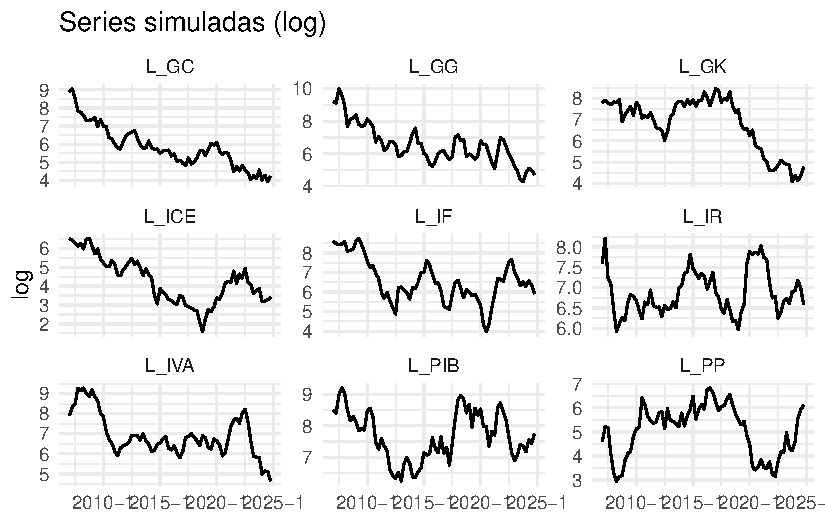
\includegraphics[keepaspectratio]{Modelos-Estructurales_files/figure-pdf/unnamed-chunk-2-1.pdf}}

\textbf{Estacionariedad en niveles y en diferencias}

\begin{Shaded}
\begin{Highlighting}[]
\NormalTok{adf\_levels }\OtherTok{\textless{}{-}} \FunctionTok{sapply}\NormalTok{(vars, }\ControlFlowTok{function}\NormalTok{(v) }\FunctionTok{adf.test}\NormalTok{(Y\_ts[,v])}\SpecialCharTok{$}\NormalTok{p.value)}
\NormalTok{adf\_diffs  }\OtherTok{\textless{}{-}} \FunctionTok{sapply}\NormalTok{(vars, }\ControlFlowTok{function}\NormalTok{(v) }\FunctionTok{adf.test}\NormalTok{(}\FunctionTok{diff}\NormalTok{(Y\_ts[,v])[}\SpecialCharTok{{-}}\DecValTok{1}\NormalTok{])}\SpecialCharTok{$}\NormalTok{p.value)}
\end{Highlighting}
\end{Shaded}

\begin{verbatim}
Warning in adf.test(diff(Y_ts[, v])[-1]): p-value smaller than printed p-value
Warning in adf.test(diff(Y_ts[, v])[-1]): p-value smaller than printed p-value
\end{verbatim}

\begin{Shaded}
\begin{Highlighting}[]
\FunctionTok{cat}\NormalTok{(}\StringTok{"}\SpecialCharTok{\textbackslash{}n}\StringTok{ADF p{-}valores en niveles:}\SpecialCharTok{\textbackslash{}n}\StringTok{"}\NormalTok{); }\FunctionTok{print}\NormalTok{(}\FunctionTok{round}\NormalTok{(adf\_levels,}\DecValTok{4}\NormalTok{))}
\end{Highlighting}
\end{Shaded}

\begin{verbatim}

ADF p-valores en niveles:
\end{verbatim}

\begin{verbatim}
  L_PP  L_PIB   L_GG   L_GC   L_GK   L_IF  L_IVA  L_ICE   L_IR 
0.5077 0.4831 0.1429 0.2622 0.8133 0.3314 0.1580 0.6756 0.1775 
\end{verbatim}

\begin{Shaded}
\begin{Highlighting}[]
\FunctionTok{cat}\NormalTok{(}\StringTok{"}\SpecialCharTok{\textbackslash{}n}\StringTok{ADF p{-}valores en diferencias:}\SpecialCharTok{\textbackslash{}n}\StringTok{"}\NormalTok{); }\FunctionTok{print}\NormalTok{(}\FunctionTok{round}\NormalTok{(adf\_diffs,}\DecValTok{4}\NormalTok{))}
\end{Highlighting}
\end{Shaded}

\begin{verbatim}

ADF p-valores en diferencias:
\end{verbatim}

\begin{verbatim}
  L_PP  L_PIB   L_GG   L_GC   L_GK   L_IF  L_IVA  L_ICE   L_IR 
0.0302 0.0100 0.0100 0.0162 0.1010 0.1381 0.1824 0.0965 0.0104 
\end{verbatim}

\subsection{\texorpdfstring{📘 \textbf{1️⃣ Hipótesis del test
ADF}}{📘 1️⃣ Hipótesis del test ADF}}\label{hipuxf3tesis-del-test-adf}

\begin{itemize}
\item
  \textbf{H₀ (nula):} La serie tiene una raíz unitaria → no
  estacionaria.
\item
  \textbf{H₁ (alternativa):} La serie es estacionaria.
\end{itemize}

\subsection{\texorpdfstring{📊 \textbf{2️⃣ Resultados por
niveles}}{📊 2️⃣ Resultados por niveles}}\label{resultados-por-niveles}

\begin{longtable}[]{@{}lll@{}}
\toprule\noalign{}
Variable & p-valor & Interpretación \\
\midrule\noalign{}
\endhead
\bottomrule\noalign{}
\endlastfoot
L\_PP & 0.5077 & No se rechaza H₀ → no estacionaria \\
L\_PIB & 0.4831 & No estacionaria \\
L\_GG & 0.1429 & No estacionaria \\
L\_GC & 0.2622 & No estacionaria \\
L\_GK & 0.8133 & No estacionaria \\
L\_IF & 0.3314 & No estacionaria \\
L\_IVA & 0.1580 & No estacionaria \\
L\_ICE & 0.6756 & No estacionaria \\
L\_IR & 0.1775 & No estacionaria \\
\end{longtable}

🔹 \textbf{Conclusión en niveles:}\\
Todas las variables tienen p-valores \textgreater{} 0.05 → \textbf{no se
rechaza la hipótesis nula de raíz unitaria}.\\
➡️ \textbf{Ninguna serie es estacionaria en niveles.}

\subsection{\texorpdfstring{📈 \textbf{3️⃣ Resultados en primeras
diferencias}}{📈 3️⃣ Resultados en primeras diferencias}}\label{resultados-en-primeras-diferencias}

\begin{longtable}[]{@{}lll@{}}
\toprule\noalign{}
Variable & p-valor & Interpretación \\
\midrule\noalign{}
\endhead
\bottomrule\noalign{}
\endlastfoot
L\_PP & 0.0302 & Estacionaria \\
L\_PIB & 0.0100 & Estacionaria \\
L\_GG & 0.0100 & Estacionaria \\
L\_GC & 0.0162 & Estacionaria \\
L\_GK & 0.1010 & No estacionaria al 5\% (pero casi) \\
L\_IF & 0.1381 & No estacionaria \\
L\_IVA & 0.1824 & No estacionaria \\
L\_ICE & 0.0965 & No estacionaria (marginal al 10\%) \\
L\_IR & 0.0104 & Estacionaria \\
\end{longtable}

🔹 \textbf{Conclusión en diferencias:}\\
La mayoría de las series

(L\_PP, L\_PIB, L\_GG, L\_GC, L\_IR)

Son estacionarias en primeras diferencias (p \textless{} 0.05).\\
Algunas (L\_GK, L\_IF, L\_IVA, L\_ICE) presentan p-valores entre
0.09--0.18, lo que podría considerarse estacionarias al 10\% o requerir
una segunda diferencia o un ajuste de rezagos.

\subsection{\texorpdfstring{\textbf{4️⃣ Implicación para el modelo
VAR}}{4️⃣ Implicación para el modelo VAR}}\label{implicaciuxf3n-para-el-modelo-var}

\begin{itemize}
\item
  Dado que las series no son estacionarias en niveles pero sí lo son en
  diferencias, se clasifican como I(1) (integradas de orden uno).
\item
  Esto sugiere que podría existir cointegración entre ellas, por lo cual
  el paso siguiente sería aplicar el test de Johansen:
\end{itemize}

\textbf{Seleccionamos los rezagos en niveles (para el Test de Johansen)}

\begin{Shaded}
\begin{Highlighting}[]
\NormalTok{sel\_lvl }\OtherTok{\textless{}{-}} \FunctionTok{VARselect}\NormalTok{(Y\_ts, }\AttributeTok{lag.max =} \DecValTok{4}\NormalTok{, }\AttributeTok{type =} \StringTok{"const"}\NormalTok{)}
\FunctionTok{cat}\NormalTok{(}\StringTok{"}\SpecialCharTok{\textbackslash{}n}\StringTok{Criterios de información (niveles):}\SpecialCharTok{\textbackslash{}n}\StringTok{"}\NormalTok{); }\FunctionTok{print}\NormalTok{(sel\_lvl}\SpecialCharTok{$}\NormalTok{criteria)}
\end{Highlighting}
\end{Shaded}

\begin{verbatim}

Criterios de información (niveles):
\end{verbatim}

\begin{verbatim}
                   1             2             3             4
AIC(n) -1.864410e+01 -1.800915e+01 -1.739430e+01 -1.776323e+01
HQ(n)  -1.748014e+01 -1.579762e+01 -1.413521e+01 -1.345658e+01
SC(n)  -1.570651e+01 -1.242774e+01 -9.169070e+00 -6.894172e+00
FPE(n)  8.153935e-09  1.731364e-08  4.454123e-08  6.316023e-08
\end{verbatim}

\begin{Shaded}
\begin{Highlighting}[]
\NormalTok{p\_opt }\OtherTok{\textless{}{-}} \FunctionTok{as.integer}\NormalTok{(sel\_lvl}\SpecialCharTok{$}\NormalTok{selection[}\StringTok{"AIC(n)"}\NormalTok{])}
\NormalTok{Kj }\OtherTok{\textless{}{-}} \FunctionTok{max}\NormalTok{(}\DecValTok{2}\NormalTok{, p\_opt)}
\FunctionTok{cat}\NormalTok{(}\StringTok{"}\SpecialCharTok{\textbackslash{}n}\StringTok{Usando K ="}\NormalTok{, Kj, }\StringTok{"para Johansen.}\SpecialCharTok{\textbackslash{}n}\StringTok{"}\NormalTok{)}
\end{Highlighting}
\end{Shaded}

\begin{verbatim}

Usando K = 2 para Johansen.
\end{verbatim}

\begin{Shaded}
\begin{Highlighting}[]
\NormalTok{j\_tr  }\OtherTok{\textless{}{-}} \FunctionTok{ca.jo}\NormalTok{(Y\_ts, }\AttributeTok{type =} \StringTok{"trace"}\NormalTok{, }\AttributeTok{K =}\NormalTok{ Kj, }\AttributeTok{ecdet =} \StringTok{"const"}\NormalTok{, }\AttributeTok{spec =} \StringTok{"transitory"}\NormalTok{)}
\NormalTok{j\_eig }\OtherTok{\textless{}{-}} \FunctionTok{ca.jo}\NormalTok{(Y\_ts, }\AttributeTok{type =} \StringTok{"eigen"}\NormalTok{, }\AttributeTok{K =}\NormalTok{ Kj, }\AttributeTok{ecdet =} \StringTok{"const"}\NormalTok{, }\AttributeTok{spec =} \StringTok{"transitory"}\NormalTok{)}
\FunctionTok{cat}\NormalTok{(}\StringTok{"}\SpecialCharTok{\textbackslash{}n}\StringTok{{-}{-}{-} Johansen TRACE {-}{-}{-}}\SpecialCharTok{\textbackslash{}n}\StringTok{"}\NormalTok{); }\FunctionTok{print}\NormalTok{(}\FunctionTok{summary}\NormalTok{(j\_tr))}
\end{Highlighting}
\end{Shaded}

\begin{verbatim}

--- Johansen TRACE ---
\end{verbatim}

\begin{verbatim}

###################### 
# Johansen-Procedure # 
###################### 

Test type: trace statistic , without linear trend and constant in cointegration 

Eigenvalues (lambda):
 [1]  5.909955e-01  4.423184e-01  3.813286e-01  3.171301e-01  2.314686e-01
 [6]  2.030888e-01  1.567262e-01  9.683625e-02  4.903297e-02 -8.006596e-17

Values of teststatistic and critical values of test:

           test  10pct   5pct   1pct
r <= 8 |   3.52   7.52   9.24  12.97
r <= 7 |  10.65  17.85  19.96  24.60
r <= 6 |  22.58  32.00  34.91  41.07
r <= 5 |  38.47  49.65  53.12  60.16
r <= 4 |  56.90  71.86  76.07  84.45
r <= 3 |  83.60  97.18 102.14 111.01
r <= 2 | 117.22 126.58 131.70 143.09
r <= 1 | 158.09 159.48 165.58 177.20
r = 0  | 220.68 196.37 202.92 215.74

Eigenvectors, normalised to first column:
(These are the cointegration relations)

             L_PP.l1    L_PIB.l1     L_GG.l1    L_GC.l1     L_GK.l1
L_PP.l1    1.0000000  1.00000000  1.00000000  1.0000000   1.0000000
L_PIB.l1   0.7324992 -2.08073054  0.06556848 -0.8190391   0.7237758
L_GG.l1   -0.2778916  3.36639420 -1.31418394 -0.2134218  -0.8948099
L_GC.l1   -0.1847404 -1.88785850 -0.48758497  1.3354645  -1.3605263
L_GK.l1   -0.2480989 -1.37287595  0.01989781 -1.0902060   0.4782761
L_IF.l1   -0.1274489  0.06782783  0.80838209 -0.3852260  -1.6148731
L_IVA.l1   0.5791197  1.20062298  1.23863346  1.4955178   1.5141218
L_ICE.l1   0.7588437 -1.09644442  0.41950093 -1.0926320   2.1507986
L_IR.l1    1.3174608 -0.32179846 -0.11028251  0.4897667   0.6610095
constant -21.3593180  7.20167336 -9.16030864 -4.6071778 -14.4253446
              L_IF.l1   L_IVA.l1   L_ICE.l1    L_IR.l1     constant
L_PP.l1    1.00000000  1.0000000  1.0000000  1.0000000  1.000000000
L_PIB.l1   2.31180164  2.1965497  0.8382612 -0.4410457  0.441582292
L_GG.l1   -0.55387332  0.1661096 -0.1437685  0.1185211 -0.563672905
L_GC.l1   -0.54347756 -0.4730255  1.6080807 -0.8404113 -0.240905965
L_GK.l1   -0.11323347  1.0887838 -1.1336760  0.9718469 -1.549307168
L_IF.l1   -0.96615237  1.3870214 -0.8986143 -1.3342308 -0.491574728
L_IVA.l1   0.97208201 -4.9683112 -0.3383076  1.9828351 -0.690720871
L_ICE.l1   0.53517813  1.8773423  1.0909467 -0.1795450  0.840946996
L_IR.l1   -0.01142896 -0.8260108 -3.7907235  0.2523096  0.009541541
constant -18.09336666 -5.5963588 18.1598105 -9.0688320 12.989079589

Weights W:
(This is the loading matrix)

             L_PP.l1     L_PIB.l1       L_GG.l1      L_GC.l1      L_GK.l1
L_PP.d  -0.170837587 -0.003662898  0.0575157278 -0.131035864  0.013545373
L_PIB.d -0.005989066 -0.017212711  0.0395195792  0.093970593 -0.008844093
L_GG.d  -0.014904228 -0.131448226  0.0984319174  0.031597461  0.065662423
L_GC.d  -0.202032138  0.037061936  0.0239556762 -0.053822660  0.023277256
L_GK.d   0.107879149  0.040323523  0.0399504908  0.097749889  0.035514573
L_IF.d  -0.130986197  0.022476659 -0.0809102756 -0.027650974  0.078040213
L_IVA.d  0.034755025 -0.021334929 -0.1195008720 -0.006213521  0.037895083
L_ICE.d -0.086456592 -0.026877165 -0.0523795313  0.110418160 -0.018931774
L_IR.d  -0.244164374 -0.033087565 -0.0007176711  0.055140201 -0.006378733
             L_IF.l1     L_IVA.l1     L_ICE.l1       L_IR.l1      constant
L_PP.d  -0.065563423 -0.012443347 -0.015033901 -0.0218652619  7.964410e-16
L_PIB.d -0.057023595  0.001508587 -0.029896084  0.0119994823 -2.777417e-17
L_GG.d   0.024103879 -0.007603056 -0.010517381  0.0042684620  2.576200e-15
L_GC.d   0.025564965  0.013161977 -0.008089357  0.0011980029  5.434942e-16
L_GK.d  -0.033141892  0.009359561  0.011561300 -0.0161955978  5.953449e-16
L_IF.d  -0.050478050 -0.015256264 -0.014706610  0.0046688332 -2.897984e-16
L_IVA.d -0.023889710  0.023095483 -0.008423701 -0.0001829324 -2.094494e-16
L_ICE.d  0.069818273 -0.004381045 -0.008119242 -0.0154794202 -1.182713e-15
L_IR.d  -0.007205277  0.003809481  0.018052746  0.0066262475 -6.074391e-16
\end{verbatim}

\begin{Shaded}
\begin{Highlighting}[]
\FunctionTok{cat}\NormalTok{(}\StringTok{"}\SpecialCharTok{\textbackslash{}n}\StringTok{{-}{-}{-} Johansen EIGEN {-}{-}{-}}\SpecialCharTok{\textbackslash{}n}\StringTok{"}\NormalTok{); }\FunctionTok{print}\NormalTok{(}\FunctionTok{summary}\NormalTok{(j\_eig))}
\end{Highlighting}
\end{Shaded}

\begin{verbatim}

--- Johansen EIGEN ---
\end{verbatim}

\begin{verbatim}

###################### 
# Johansen-Procedure # 
###################### 

Test type: maximal eigenvalue statistic (lambda max) , without linear trend and constant in cointegration 

Eigenvalues (lambda):
 [1]  5.909955e-01  4.423184e-01  3.813286e-01  3.171301e-01  2.314686e-01
 [6]  2.030888e-01  1.567262e-01  9.683625e-02  4.903297e-02 -8.006596e-17

Values of teststatistic and critical values of test:

          test 10pct  5pct  1pct
r <= 8 |  3.52  7.52  9.24 12.97
r <= 7 |  7.13 13.75 15.67 20.20
r <= 6 | 11.93 19.77 22.00 26.81
r <= 5 | 15.89 25.56 28.14 33.24
r <= 4 | 18.43 31.66 34.40 39.79
r <= 3 | 26.70 37.45 40.30 46.82
r <= 2 | 33.61 43.25 46.45 51.91
r <= 1 | 40.88 48.91 52.00 57.95
r = 0  | 62.58 54.35 57.42 63.71

Eigenvectors, normalised to first column:
(These are the cointegration relations)

             L_PP.l1    L_PIB.l1     L_GG.l1    L_GC.l1     L_GK.l1
L_PP.l1    1.0000000  1.00000000  1.00000000  1.0000000   1.0000000
L_PIB.l1   0.7324992 -2.08073054  0.06556848 -0.8190391   0.7237758
L_GG.l1   -0.2778916  3.36639420 -1.31418394 -0.2134218  -0.8948099
L_GC.l1   -0.1847404 -1.88785850 -0.48758497  1.3354645  -1.3605263
L_GK.l1   -0.2480989 -1.37287595  0.01989781 -1.0902060   0.4782761
L_IF.l1   -0.1274489  0.06782783  0.80838209 -0.3852260  -1.6148731
L_IVA.l1   0.5791197  1.20062298  1.23863346  1.4955178   1.5141218
L_ICE.l1   0.7588437 -1.09644442  0.41950093 -1.0926320   2.1507986
L_IR.l1    1.3174608 -0.32179846 -0.11028251  0.4897667   0.6610095
constant -21.3593180  7.20167336 -9.16030864 -4.6071778 -14.4253446
              L_IF.l1   L_IVA.l1   L_ICE.l1    L_IR.l1     constant
L_PP.l1    1.00000000  1.0000000  1.0000000  1.0000000  1.000000000
L_PIB.l1   2.31180164  2.1965497  0.8382612 -0.4410457  0.441582292
L_GG.l1   -0.55387332  0.1661096 -0.1437685  0.1185211 -0.563672905
L_GC.l1   -0.54347756 -0.4730255  1.6080807 -0.8404113 -0.240905965
L_GK.l1   -0.11323347  1.0887838 -1.1336760  0.9718469 -1.549307168
L_IF.l1   -0.96615237  1.3870214 -0.8986143 -1.3342308 -0.491574728
L_IVA.l1   0.97208201 -4.9683112 -0.3383076  1.9828351 -0.690720871
L_ICE.l1   0.53517813  1.8773423  1.0909467 -0.1795450  0.840946996
L_IR.l1   -0.01142896 -0.8260108 -3.7907235  0.2523096  0.009541541
constant -18.09336666 -5.5963588 18.1598105 -9.0688320 12.989079589

Weights W:
(This is the loading matrix)

             L_PP.l1     L_PIB.l1       L_GG.l1      L_GC.l1      L_GK.l1
L_PP.d  -0.170837587 -0.003662898  0.0575157278 -0.131035864  0.013545373
L_PIB.d -0.005989066 -0.017212711  0.0395195792  0.093970593 -0.008844093
L_GG.d  -0.014904228 -0.131448226  0.0984319174  0.031597461  0.065662423
L_GC.d  -0.202032138  0.037061936  0.0239556762 -0.053822660  0.023277256
L_GK.d   0.107879149  0.040323523  0.0399504908  0.097749889  0.035514573
L_IF.d  -0.130986197  0.022476659 -0.0809102756 -0.027650974  0.078040213
L_IVA.d  0.034755025 -0.021334929 -0.1195008720 -0.006213521  0.037895083
L_ICE.d -0.086456592 -0.026877165 -0.0523795313  0.110418160 -0.018931774
L_IR.d  -0.244164374 -0.033087565 -0.0007176711  0.055140201 -0.006378733
             L_IF.l1     L_IVA.l1     L_ICE.l1       L_IR.l1      constant
L_PP.d  -0.065563423 -0.012443347 -0.015033901 -0.0218652619  7.964410e-16
L_PIB.d -0.057023595  0.001508587 -0.029896084  0.0119994823 -2.777417e-17
L_GG.d   0.024103879 -0.007603056 -0.010517381  0.0042684620  2.576200e-15
L_GC.d   0.025564965  0.013161977 -0.008089357  0.0011980029  5.434942e-16
L_GK.d  -0.033141892  0.009359561  0.011561300 -0.0161955978  5.953449e-16
L_IF.d  -0.050478050 -0.015256264 -0.014706610  0.0046688332 -2.897984e-16
L_IVA.d -0.023889710  0.023095483 -0.008423701 -0.0001829324 -2.094494e-16
L_ICE.d  0.069818273 -0.004381045 -0.008119242 -0.0154794202 -1.182713e-15
L_IR.d  -0.007205277  0.003809481  0.018052746  0.0066262475 -6.074391e-16
\end{verbatim}

\begin{Shaded}
\begin{Highlighting}[]
\NormalTok{choose\_r\_trace }\OtherTok{\textless{}{-}} \ControlFlowTok{function}\NormalTok{(jobj, }\AttributeTok{alpha =} \FloatTok{0.05}\NormalTok{) \{}
\NormalTok{  ts }\OtherTok{\textless{}{-}}\NormalTok{ jobj}\SpecialCharTok{@}\NormalTok{teststat}
\NormalTok{  cv }\OtherTok{\textless{}{-}}\NormalTok{ jobj}\SpecialCharTok{@}\NormalTok{cval[,}\StringTok{"5pct"}\NormalTok{]}
  \FunctionTok{sum}\NormalTok{(ts }\SpecialCharTok{\textgreater{}}\NormalTok{ cv)}
\NormalTok{\}}
\NormalTok{r }\OtherTok{\textless{}{-}} \FunctionTok{max}\NormalTok{(}\DecValTok{1}\NormalTok{, }\FunctionTok{choose\_r\_trace}\NormalTok{(j\_tr, }\FloatTok{0.05}\NormalTok{))   }\CommentTok{\# asegura r≥1 para poder estimar VECM}
\FunctionTok{cat}\NormalTok{(}\StringTok{"}\SpecialCharTok{\textbackslash{}n}\StringTok{Rango de cointegración estimado (trace, 5\%): r ="}\NormalTok{, r, }\StringTok{"}\SpecialCharTok{\textbackslash{}n}\StringTok{"}\NormalTok{)}
\end{Highlighting}
\end{Shaded}

\begin{verbatim}

Rango de cointegración estimado (trace, 5%): r = 1 
\end{verbatim}

La salida proviene de la selección del número óptimo de rezagos \((p)\)
en un modelo VAR.\\

Los criterios de información (AIC, HQ, SC, FPE) comparan la bondad de
ajuste y la penalización por complejidad del modelo (número de rezagos).

El objetivo es elegir el valor de \((p)\) que minimiza el criterio
seleccionado.

-Normalmente \textbf{AIC} (Akaike Information Criterion) o
\textbf{BIC/SC} (Schwarz Criterion).

\begin{Shaded}
\begin{Highlighting}[]
\NormalTok{vecm\_fit }\OtherTok{\textless{}{-}} \FunctionTok{cajorls}\NormalTok{(j\_tr, }\AttributeTok{r =}\NormalTok{ r)}
\FunctionTok{cat}\NormalTok{(}\StringTok{"}\SpecialCharTok{\textbackslash{}n}\StringTok{{-}{-}{-} Beta (vectores cointegrados estimados) {-}{-}{-}}\SpecialCharTok{\textbackslash{}n}\StringTok{"}\NormalTok{)}
\end{Highlighting}
\end{Shaded}

\begin{verbatim}

--- Beta (vectores cointegrados estimados) ---
\end{verbatim}

\begin{Shaded}
\begin{Highlighting}[]
\FunctionTok{print}\NormalTok{(vecm\_fit}\SpecialCharTok{$}\NormalTok{beta)}
\end{Highlighting}
\end{Shaded}

\begin{verbatim}
                ect1
L_PP.l1    1.0000000
L_PIB.l1   0.7324992
L_GG.l1   -0.2778916
L_GC.l1   -0.1847404
L_GK.l1   -0.2480989
L_IF.l1   -0.1274489
L_IVA.l1   0.5791197
L_ICE.l1   0.7588437
L_IR.l1    1.3174608
constant -21.3593180
\end{verbatim}

\begin{Shaded}
\begin{Highlighting}[]
\NormalTok{var\_from\_vecm }\OtherTok{\textless{}{-}} \FunctionTok{vec2var}\NormalTok{(j\_tr, }\AttributeTok{r =}\NormalTok{ r)  }
\end{Highlighting}
\end{Shaded}

Función para elejir r 5\%

\begin{Shaded}
\begin{Highlighting}[]
\FunctionTok{cat}\NormalTok{(}\StringTok{"}\SpecialCharTok{\textbackslash{}n}\StringTok{{-}{-}{-} Portmanteau {-}{-}{-}}\SpecialCharTok{\textbackslash{}n}\StringTok{"}\NormalTok{); }\FunctionTok{print}\NormalTok{(}\FunctionTok{serial.test}\NormalTok{(var\_from\_vecm, }\AttributeTok{lags.pt =} \DecValTok{12}\NormalTok{, }\AttributeTok{type =} \StringTok{"PT.asymptotic"}\NormalTok{))}
\end{Highlighting}
\end{Shaded}

\begin{verbatim}

--- Portmanteau ---
\end{verbatim}

\begin{verbatim}

    Portmanteau Test (asymptotic)

data:  Residuals of VAR object var_from_vecm
Chi-squared = 854.21, df = 819, p-value = 0.191
\end{verbatim}

\begin{verbatim}
$serial

    Portmanteau Test (asymptotic)

data:  Residuals of VAR object var_from_vecm
Chi-squared = 854.21, df = 819, p-value = 0.191
\end{verbatim}

\begin{Shaded}
\begin{Highlighting}[]
\FunctionTok{cat}\NormalTok{(}\StringTok{"}\SpecialCharTok{\textbackslash{}n}\StringTok{{-}{-}{-} ARCH {-}{-}{-}}\SpecialCharTok{\textbackslash{}n}\StringTok{"}\NormalTok{); }\FunctionTok{print}\NormalTok{(}\FunctionTok{arch.test}\NormalTok{(var\_from\_vecm, }\AttributeTok{lags.multi =} \DecValTok{5}\NormalTok{))}
\end{Highlighting}
\end{Shaded}

\begin{verbatim}

--- ARCH ---
\end{verbatim}

\begin{verbatim}

    ARCH (multivariate)

data:  Residuals of VAR object var_from_vecm
Chi-squared = 2925, df = 10125, p-value = 1
\end{verbatim}

\begin{verbatim}
$arch.mul

    ARCH (multivariate)

data:  Residuals of VAR object var_from_vecm
Chi-squared = 2925, df = 10125, p-value = 1
\end{verbatim}

\begin{Shaded}
\begin{Highlighting}[]
\FunctionTok{cat}\NormalTok{(}\StringTok{"}\SpecialCharTok{\textbackslash{}n}\StringTok{{-}{-}{-} Normalidad {-}{-}{-}}\SpecialCharTok{\textbackslash{}n}\StringTok{"}\NormalTok{); }\FunctionTok{print}\NormalTok{(}\FunctionTok{normality.test}\NormalTok{(var\_from\_vecm))}
\end{Highlighting}
\end{Shaded}

\begin{verbatim}

--- Normalidad ---
\end{verbatim}

\begin{verbatim}
$JB

    JB-Test (multivariate)

data:  Residuals of VAR object var_from_vecm
Chi-squared = 12.03, df = 18, p-value = 0.8457


$Skewness

    Skewness only (multivariate)

data:  Residuals of VAR object var_from_vecm
Chi-squared = 7.3634, df = 9, p-value = 0.5993


$Kurtosis

    Kurtosis only (multivariate)

data:  Residuals of VAR object var_from_vecm
Chi-squared = 4.6671, df = 9, p-value = 0.8623
\end{verbatim}

\begin{verbatim}
$jb.mul
$jb.mul$JB

    JB-Test (multivariate)

data:  Residuals of VAR object var_from_vecm
Chi-squared = 12.03, df = 18, p-value = 0.8457


$jb.mul$Skewness

    Skewness only (multivariate)

data:  Residuals of VAR object var_from_vecm
Chi-squared = 7.3634, df = 9, p-value = 0.5993


$jb.mul$Kurtosis

    Kurtosis only (multivariate)

data:  Residuals of VAR object var_from_vecm
Chi-squared = 4.6671, df = 9, p-value = 0.8623
\end{verbatim}

\textbf{Estimación Estabilidad}

\begin{Shaded}
\begin{Highlighting}[]
\NormalTok{var\_levels }\OtherTok{\textless{}{-}} \FunctionTok{VAR}\NormalTok{(Y\_ts, }\AttributeTok{p =}\NormalTok{ Kj, }\AttributeTok{type =} \StringTok{"const"}\NormalTok{)}
\NormalTok{mod\_roots }\OtherTok{\textless{}{-}} \FunctionTok{roots}\NormalTok{(var\_levels, }\AttributeTok{modulus =} \ConstantTok{TRUE}\NormalTok{)}
\FunctionTok{cat}\NormalTok{(}\StringTok{"}\SpecialCharTok{\textbackslash{}n}\StringTok{Módulos de autovalores (VAR en niveles, p=Kj):}\SpecialCharTok{\textbackslash{}n}\StringTok{"}\NormalTok{); }\FunctionTok{print}\NormalTok{(}\FunctionTok{round}\NormalTok{(}\FunctionTok{sort}\NormalTok{(mod\_roots, }\AttributeTok{decreasing =} \ConstantTok{TRUE}\NormalTok{), }\DecValTok{4}\NormalTok{))}
\end{Highlighting}
\end{Shaded}

\begin{verbatim}

Módulos de autovalores (VAR en niveles, p=Kj):
\end{verbatim}

\begin{verbatim}
 [1] 0.9700 0.9390 0.9390 0.9112 0.9112 0.7489 0.7489 0.6939 0.6939 0.5709
[11] 0.5709 0.4576 0.4576 0.3993 0.2880 0.1840 0.1840 0.0639
\end{verbatim}

\begin{Shaded}
\begin{Highlighting}[]
\FunctionTok{plot}\NormalTok{(}\FunctionTok{roots}\NormalTok{(var\_levels))   }\CommentTok{\# puntos dentro del círculo =\textgreater{} estable}
\end{Highlighting}
\end{Shaded}

\pandocbounded{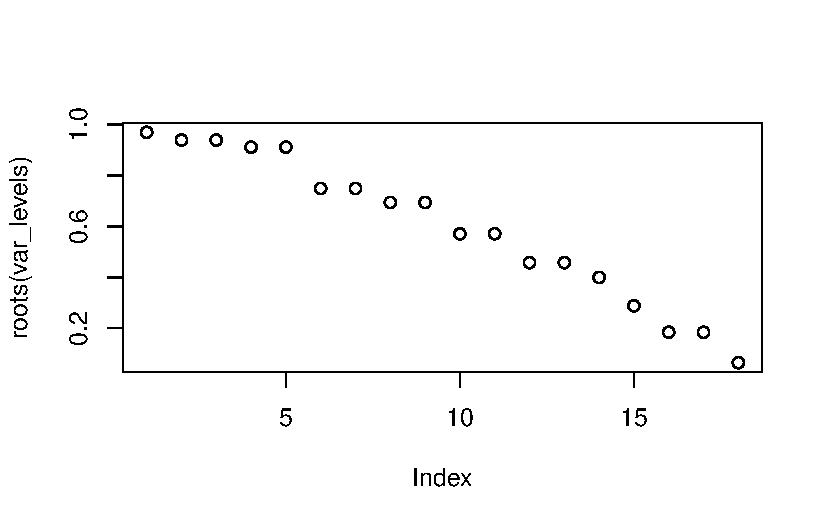
\includegraphics[keepaspectratio]{Modelos-Estructurales_files/figure-pdf/unnamed-chunk-7-1.pdf}}

\subsection{VAR equivalente del VECM (para
IRF/FEVD/forecast)}\label{var-equivalente-del-vecm-para-irffevdforecast}

\begin{Shaded}
\begin{Highlighting}[]
\NormalTok{dY\_ts }\OtherTok{\textless{}{-}} \FunctionTok{na.omit}\NormalTok{(}\FunctionTok{diff}\NormalTok{(Y\_ts))}
\NormalTok{sel\_d }\OtherTok{\textless{}{-}} \FunctionTok{VARselect}\NormalTok{(dY\_ts, }\AttributeTok{lag.max =} \DecValTok{4}\NormalTok{, }\AttributeTok{type =} \StringTok{"const"}\NormalTok{)}
\NormalTok{p\_d }\OtherTok{\textless{}{-}} \FunctionTok{ifelse}\NormalTok{(}\FunctionTok{is.na}\NormalTok{(}\FunctionTok{as.integer}\NormalTok{(sel\_d}\SpecialCharTok{$}\NormalTok{selection[}\StringTok{"AIC(n)"}\NormalTok{])), }\DecValTok{2}\NormalTok{L, }\FunctionTok{as.integer}\NormalTok{(sel\_d}\SpecialCharTok{$}\NormalTok{selection[}\StringTok{"AIC(n)"}\NormalTok{]))}
\FunctionTok{cat}\NormalTok{(}\StringTok{"}\SpecialCharTok{\textbackslash{}n}\StringTok{VAR(Δ) seleccionado (AIC): p\_d ="}\NormalTok{, p\_d, }\StringTok{"}\SpecialCharTok{\textbackslash{}n}\StringTok{"}\NormalTok{)}
\end{Highlighting}
\end{Shaded}

\begin{verbatim}

VAR(Δ) seleccionado (AIC): p_d = 1 
\end{verbatim}

\begin{Shaded}
\begin{Highlighting}[]
\NormalTok{var\_d }\OtherTok{\textless{}{-}} \FunctionTok{VAR}\NormalTok{(dY\_ts, }\AttributeTok{p =}\NormalTok{ p\_d, }\AttributeTok{type =} \StringTok{"const"}\NormalTok{)}
\NormalTok{stb\_diff }\OtherTok{\textless{}{-}} \FunctionTok{stability}\NormalTok{(var\_d, }\AttributeTok{type =} \StringTok{"OLS{-}CUSUM"}\NormalTok{)}
\end{Highlighting}
\end{Shaded}

\begin{Shaded}
\begin{Highlighting}[]
\FunctionTok{png}\NormalTok{(}\StringTok{"stability\_VAR\_diff\_CUSUM.png"}\NormalTok{, }\AttributeTok{width =} \DecValTok{1400}\NormalTok{, }\AttributeTok{height =} \DecValTok{900}\NormalTok{, }\AttributeTok{res =} \DecValTok{150}\NormalTok{)}
\FunctionTok{par}\NormalTok{(}\AttributeTok{mar =} \FunctionTok{c}\NormalTok{(}\DecValTok{4}\NormalTok{, }\DecValTok{4}\NormalTok{, }\DecValTok{2}\NormalTok{, }\DecValTok{1}\NormalTok{))}
\FunctionTok{plot}\NormalTok{(stb\_diff)}
\FunctionTok{dev.off}\NormalTok{()}
\end{Highlighting}
\end{Shaded}

\begin{verbatim}
pdf 
  2 
\end{verbatim}

\begin{Shaded}
\begin{Highlighting}[]
\FunctionTok{cat}\NormalTok{(}\StringTok{"Gráfico guardado en: stability\_VAR\_diff\_CUSUM.png}\SpecialCharTok{\textbackslash{}n}\StringTok{"}\NormalTok{)}
\end{Highlighting}
\end{Shaded}

\begin{verbatim}
Gráfico guardado en: stability_VAR_diff_CUSUM.png
\end{verbatim}

\textbf{IRF}

\begin{Shaded}
\begin{Highlighting}[]
\NormalTok{irf\_pp\_pib }\OtherTok{\textless{}{-}} \FunctionTok{irf}\NormalTok{(var\_from\_vecm, }\AttributeTok{impulse =} \StringTok{"L\_PP"}\NormalTok{, }\AttributeTok{response =} \StringTok{"L\_PIB"}\NormalTok{,}
                  \AttributeTok{n.ahead =} \DecValTok{12}\NormalTok{, }\AttributeTok{boot =} \ConstantTok{TRUE}\NormalTok{, }\AttributeTok{ci =} \FloatTok{0.95}\NormalTok{)}
\FunctionTok{plot}\NormalTok{(irf\_pp\_pib)}
\end{Highlighting}
\end{Shaded}

\pandocbounded{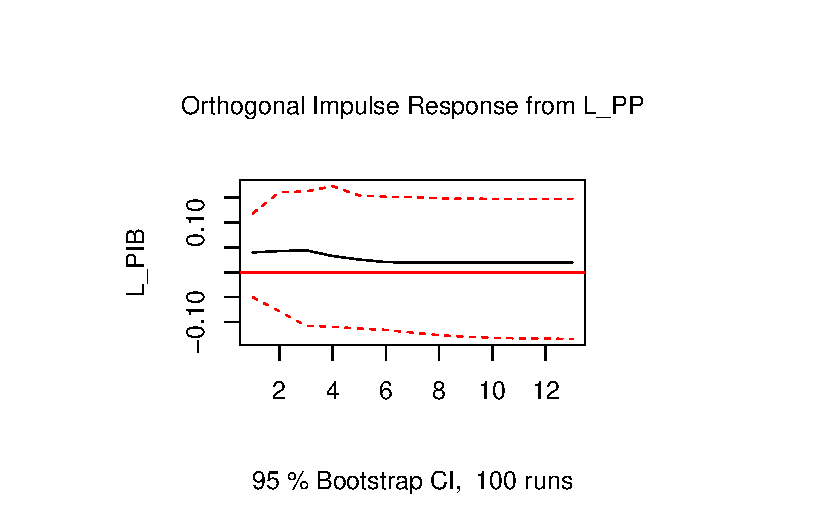
\includegraphics[keepaspectratio]{Modelos-Estructurales_files/figure-pdf/unnamed-chunk-10-1.pdf}}

\begin{Shaded}
\begin{Highlighting}[]
\NormalTok{fevd\_v }\OtherTok{\textless{}{-}} \FunctionTok{fevd}\NormalTok{(var\_from\_vecm, }\AttributeTok{n.ahead =} \DecValTok{12}\NormalTok{)}


\CommentTok{\# Cierra cualquier gráfico abierto}
\ControlFlowTok{while}\NormalTok{ (}\SpecialCharTok{!}\FunctionTok{is.null}\NormalTok{(}\FunctionTok{dev.list}\NormalTok{())) }\FunctionTok{dev.off}\NormalTok{()}

\CommentTok{\# Exporta el FEVD a un PNG}
\FunctionTok{png}\NormalTok{(}\StringTok{"FEVD\_VECM.png"}\NormalTok{, }\AttributeTok{width =} \DecValTok{1400}\NormalTok{, }\AttributeTok{height =} \DecValTok{900}\NormalTok{, }\AttributeTok{res =} \DecValTok{150}\NormalTok{)}
\FunctionTok{par}\NormalTok{(}\AttributeTok{mar =} \FunctionTok{c}\NormalTok{(}\DecValTok{4}\NormalTok{,}\DecValTok{4}\NormalTok{,}\DecValTok{2}\NormalTok{,}\DecValTok{1}\NormalTok{))  }\CommentTok{\# Márgenes reducidas}
\FunctionTok{plot}\NormalTok{(fevd\_v)}
\FunctionTok{dev.off}\NormalTok{()}
\end{Highlighting}
\end{Shaded}

\begin{verbatim}
pdf 
  2 
\end{verbatim}

\begin{Shaded}
\begin{Highlighting}[]
\FunctionTok{cat}\NormalTok{(}\StringTok{"✅ Gráfico FEVD guardado como \textquotesingle{}FEVD\_VECM.png\textquotesingle{} en tu directorio de trabajo.}\SpecialCharTok{\textbackslash{}n}\StringTok{"}\NormalTok{)}
\end{Highlighting}
\end{Shaded}

\begin{verbatim}
✅ Gráfico FEVD guardado como 'FEVD_VECM.png' en tu directorio de trabajo.
\end{verbatim}

\begin{Shaded}
\begin{Highlighting}[]
\CommentTok{\# IRF: L\_PP → L\_PIB}
\FunctionTok{png}\NormalTok{(}\StringTok{"IRF\_L\_PP\_to\_L\_PIB.png"}\NormalTok{, }\AttributeTok{width =} \DecValTok{1400}\NormalTok{, }\AttributeTok{height =} \DecValTok{900}\NormalTok{, }\AttributeTok{res =} \DecValTok{150}\NormalTok{)}
\FunctionTok{par}\NormalTok{(}\AttributeTok{mar =} \FunctionTok{c}\NormalTok{(}\DecValTok{4}\NormalTok{,}\DecValTok{4}\NormalTok{,}\DecValTok{2}\NormalTok{,}\DecValTok{1}\NormalTok{))}
\FunctionTok{plot}\NormalTok{(irf\_pp\_pib)}
\FunctionTok{dev.off}\NormalTok{()}
\end{Highlighting}
\end{Shaded}

\begin{verbatim}
pdf 
  2 
\end{verbatim}

\begin{Shaded}
\begin{Highlighting}[]
\FunctionTok{cat}\NormalTok{(}\StringTok{"✅ Gráfico IRF guardado como \textquotesingle{}IRF\_L\_PP\_to\_L\_PIB.png\textquotesingle{}}\SpecialCharTok{\textbackslash{}n}\StringTok{"}\NormalTok{)}
\end{Highlighting}
\end{Shaded}

\begin{verbatim}
✅ Gráfico IRF guardado como 'IRF_L_PP_to_L_PIB.png'
\end{verbatim}

\subsection{\texorpdfstring{\textbf{Modelo
SVAR}}{Modelo SVAR}}\label{modelo-svar}

\begin{Shaded}
\begin{Highlighting}[]
\CommentTok{\# =========================================================}
\CommentTok{\# 0) Paquetes y setup}
\CommentTok{\# =========================================================}
\CommentTok{\# install.packages(c("zoo","ggplot2","tseries","vars","urca","forecast","dplyr","tidyr"))}
\FunctionTok{library}\NormalTok{(zoo)}
\FunctionTok{library}\NormalTok{(ggplot2)}
\FunctionTok{library}\NormalTok{(tseries)}
\FunctionTok{library}\NormalTok{(vars)}
\FunctionTok{library}\NormalTok{(urca)}
\FunctionTok{library}\NormalTok{(forecast)}
\FunctionTok{library}\NormalTok{(dplyr)}
\FunctionTok{library}\NormalTok{(tidyr)}

\FunctionTok{set.seed}\NormalTok{(}\DecValTok{42}\NormalTok{)}

\CommentTok{\# =========================================================}
\CommentTok{\# 1) Calendario y variables (72 trimestres 2007Q1–2024Q4)}
\CommentTok{\# =========================================================}
\NormalTok{T  }\OtherTok{\textless{}{-}} \DecValTok{72}
\NormalTok{fq }\OtherTok{\textless{}{-}} \DecValTok{4}
\NormalTok{fechas }\OtherTok{\textless{}{-}} \FunctionTok{as.yearqtr}\NormalTok{(}\FunctionTok{seq}\NormalTok{(}\AttributeTok{from =} \FunctionTok{as.Date}\NormalTok{(}\StringTok{"2007{-}01{-}01"}\NormalTok{),}
                         \AttributeTok{by =} \StringTok{"quarter"}\NormalTok{, }\AttributeTok{length.out =}\NormalTok{ T))}
\NormalTok{vars }\OtherTok{\textless{}{-}} \FunctionTok{c}\NormalTok{(}\StringTok{"L\_PP"}\NormalTok{,}\StringTok{"L\_PIB"}\NormalTok{,}\StringTok{"L\_GG"}\NormalTok{,}\StringTok{"L\_GC"}\NormalTok{,}\StringTok{"L\_GK"}\NormalTok{,}\StringTok{"L\_IF"}\NormalTok{,}\StringTok{"L\_IVA"}\NormalTok{,}\StringTok{"L\_ICE"}\NormalTok{,}\StringTok{"L\_IR"}\NormalTok{)}
\NormalTok{k }\OtherTok{\textless{}{-}} \FunctionTok{length}\NormalTok{(vars)}

\CommentTok{\# =========================================================}
\CommentTok{\# 2) DGP: I(1) con 2 cointegraciones plausibles (para simular)}
\CommentTok{\# =========================================================}
\NormalTok{beta }\OtherTok{\textless{}{-}} \FunctionTok{matrix}\NormalTok{(}\DecValTok{0}\NormalTok{, }\AttributeTok{nrow =}\NormalTok{ k, }\AttributeTok{ncol =} \DecValTok{2}\NormalTok{, }\AttributeTok{dimnames =} \FunctionTok{list}\NormalTok{(vars, }\FunctionTok{c}\NormalTok{(}\StringTok{"CI\_gasto"}\NormalTok{,}\StringTok{"CI\_tributos"}\NormalTok{)))}
\NormalTok{beta[}\StringTok{"L\_GG"}\NormalTok{,}\StringTok{"CI\_gasto"}\NormalTok{] }\OtherTok{\textless{}{-}} \DecValTok{1}\NormalTok{;   beta[}\StringTok{"L\_GC"}\NormalTok{,}\StringTok{"CI\_gasto"}\NormalTok{] }\OtherTok{\textless{}{-}} \SpecialCharTok{{-}}\FloatTok{0.7}\NormalTok{; beta[}\StringTok{"L\_GK"}\NormalTok{,}\StringTok{"CI\_gasto"}\NormalTok{] }\OtherTok{\textless{}{-}} \SpecialCharTok{{-}}\FloatTok{0.3}
\NormalTok{beta[}\StringTok{"L\_IF"}\NormalTok{,}\StringTok{"CI\_tributos"}\NormalTok{] }\OtherTok{\textless{}{-}} \DecValTok{1}\NormalTok{; beta[}\StringTok{"L\_IVA"}\NormalTok{,}\StringTok{"CI\_tributos"}\NormalTok{] }\OtherTok{\textless{}{-}} \SpecialCharTok{{-}}\FloatTok{0.5}\NormalTok{; beta[}\StringTok{"L\_IR"}\NormalTok{,}\StringTok{"CI\_tributos"}\NormalTok{] }\OtherTok{\textless{}{-}} \SpecialCharTok{{-}}\FloatTok{0.3}\NormalTok{; beta[}\StringTok{"L\_ICE"}\NormalTok{,}\StringTok{"CI\_tributos"}\NormalTok{] }\OtherTok{\textless{}{-}} \SpecialCharTok{{-}}\FloatTok{0.2}

\NormalTok{alpha }\OtherTok{\textless{}{-}} \FunctionTok{matrix}\NormalTok{(}\DecValTok{0}\NormalTok{, }\AttributeTok{nrow =}\NormalTok{ k, }\AttributeTok{ncol =} \DecValTok{2}\NormalTok{, }\AttributeTok{dimnames =} \FunctionTok{list}\NormalTok{(vars, }\FunctionTok{c}\NormalTok{(}\StringTok{"CI\_gasto"}\NormalTok{,}\StringTok{"CI\_tributos"}\NormalTok{)))}
\NormalTok{alpha[}\StringTok{"L\_GG"}\NormalTok{,}\StringTok{"CI\_gasto"}\NormalTok{]  }\OtherTok{\textless{}{-}} \SpecialCharTok{{-}}\FloatTok{0.25}
\NormalTok{alpha[}\StringTok{"L\_GC"}\NormalTok{,}\StringTok{"CI\_gasto"}\NormalTok{]  }\OtherTok{\textless{}{-}} \SpecialCharTok{{-}}\FloatTok{0.10}
\NormalTok{alpha[}\StringTok{"L\_GK"}\NormalTok{,}\StringTok{"CI\_gasto"}\NormalTok{]  }\OtherTok{\textless{}{-}} \SpecialCharTok{{-}}\FloatTok{0.05}
\NormalTok{alpha[}\StringTok{"L\_IF"}\NormalTok{,}\StringTok{"CI\_tributos"}\NormalTok{]  }\OtherTok{\textless{}{-}} \SpecialCharTok{{-}}\FloatTok{0.20}
\NormalTok{alpha[}\StringTok{"L\_IVA"}\NormalTok{,}\StringTok{"CI\_tributos"}\NormalTok{] }\OtherTok{\textless{}{-}} \SpecialCharTok{{-}}\FloatTok{0.10}
\NormalTok{alpha[}\StringTok{"L\_IR"}\NormalTok{,}\StringTok{"CI\_tributos"}\NormalTok{]  }\OtherTok{\textless{}{-}} \SpecialCharTok{{-}}\FloatTok{0.08}
\NormalTok{alpha[}\StringTok{"L\_ICE"}\NormalTok{,}\StringTok{"CI\_tributos"}\NormalTok{] }\OtherTok{\textless{}{-}} \SpecialCharTok{{-}}\FloatTok{0.05}
\NormalTok{alpha[}\StringTok{"L\_PIB"}\NormalTok{,}\StringTok{"CI\_gasto"}\NormalTok{]    }\OtherTok{\textless{}{-}} \SpecialCharTok{{-}}\FloatTok{0.02}
\NormalTok{alpha[}\StringTok{"L\_PIB"}\NormalTok{,}\StringTok{"CI\_tributos"}\NormalTok{] }\OtherTok{\textless{}{-}} \SpecialCharTok{{-}}\FloatTok{0.01}
\NormalTok{alpha[}\StringTok{"L\_PP"}\NormalTok{,] }\OtherTok{\textless{}{-}} \FunctionTok{c}\NormalTok{(}\DecValTok{0}\NormalTok{,}\DecValTok{0}\NormalTok{)  }\CommentTok{\# petróleo no corrige directamente}

\NormalTok{Gamma1 }\OtherTok{\textless{}{-}} \FunctionTok{matrix}\NormalTok{(}\DecValTok{0}\NormalTok{, }\AttributeTok{nrow =}\NormalTok{ k, }\AttributeTok{ncol =}\NormalTok{ k, }\AttributeTok{dimnames =} \FunctionTok{list}\NormalTok{(vars, vars))}
\NormalTok{Gamma1[}\StringTok{"L\_PIB"}\NormalTok{,}\StringTok{"L\_PP"}\NormalTok{] }\OtherTok{\textless{}{-}} \FloatTok{0.10}
\NormalTok{Gamma1[}\StringTok{"L\_IF"}\NormalTok{,}\StringTok{"L\_PP"}\NormalTok{]  }\OtherTok{\textless{}{-}} \FloatTok{0.08}
\NormalTok{Gamma1[}\StringTok{"L\_IF"}\NormalTok{,}\StringTok{"L\_IVA"}\NormalTok{] }\OtherTok{\textless{}{-}} \FloatTok{0.10}\NormalTok{; Gamma1[}\StringTok{"L\_IF"}\NormalTok{,}\StringTok{"L\_IR"}\NormalTok{] }\OtherTok{\textless{}{-}} \FloatTok{0.07}\NormalTok{; Gamma1[}\StringTok{"L\_IF"}\NormalTok{,}\StringTok{"L\_ICE"}\NormalTok{] }\OtherTok{\textless{}{-}} \FloatTok{0.05}
\NormalTok{Gamma1[}\StringTok{"L\_GG"}\NormalTok{,}\StringTok{"L\_PIB"}\NormalTok{] }\OtherTok{\textless{}{-}} \FloatTok{0.06}
\NormalTok{Gamma1[}\StringTok{"L\_GC"}\NormalTok{,}\StringTok{"L\_GG"}\NormalTok{]  }\OtherTok{\textless{}{-}} \FloatTok{0.10}
\NormalTok{Gamma1[}\StringTok{"L\_GK"}\NormalTok{,}\StringTok{"L\_GG"}\NormalTok{]  }\OtherTok{\textless{}{-}} \FloatTok{0.06}

\NormalTok{Sigma }\OtherTok{\textless{}{-}} \FunctionTok{diag}\NormalTok{(}\FunctionTok{c}\NormalTok{(}\FloatTok{0.20}\NormalTok{, }\FloatTok{0.18}\NormalTok{, }\FloatTok{0.15}\NormalTok{, }\FloatTok{0.12}\NormalTok{, }\FloatTok{0.12}\NormalTok{, }\FloatTok{0.18}\NormalTok{, }\FloatTok{0.15}\NormalTok{, }\FloatTok{0.12}\NormalTok{, }\FloatTok{0.12}\NormalTok{))}
\FunctionTok{dimnames}\NormalTok{(Sigma) }\OtherTok{\textless{}{-}} \FunctionTok{list}\NormalTok{(vars, vars)}
\NormalTok{Sigma[}\StringTok{"L\_PIB"}\NormalTok{,}\StringTok{"L\_PP"}\NormalTok{] }\OtherTok{\textless{}{-}}\NormalTok{ Sigma[}\StringTok{"L\_PP"}\NormalTok{,}\StringTok{"L\_PIB"}\NormalTok{] }\OtherTok{\textless{}{-}} \FloatTok{0.05}
\NormalTok{Sigma[}\StringTok{"L\_IF"}\NormalTok{,}\StringTok{"L\_PP"}\NormalTok{]  }\OtherTok{\textless{}{-}}\NormalTok{ Sigma[}\StringTok{"L\_PP"}\NormalTok{,}\StringTok{"L\_IF"}\NormalTok{]  }\OtherTok{\textless{}{-}} \FloatTok{0.04}
\NormalTok{Sigma[}\StringTok{"L\_IF"}\NormalTok{,}\StringTok{"L\_IVA"}\NormalTok{] }\OtherTok{\textless{}{-}}\NormalTok{ Sigma[}\StringTok{"L\_IVA"}\NormalTok{,}\StringTok{"L\_IF"}\NormalTok{] }\OtherTok{\textless{}{-}} \FloatTok{0.06}
\NormalTok{Sigma[}\StringTok{"L\_GG"}\NormalTok{,}\StringTok{"L\_PIB"}\NormalTok{] }\OtherTok{\textless{}{-}}\NormalTok{ Sigma[}\StringTok{"L\_PIB"}\NormalTok{,}\StringTok{"L\_GG"}\NormalTok{] }\OtherTok{\textless{}{-}} \FloatTok{0.04}
\NormalTok{Sigma }\OtherTok{\textless{}{-}}\NormalTok{ (Sigma }\SpecialCharTok{+} \FunctionTok{t}\NormalTok{(Sigma))}\SpecialCharTok{/}\DecValTok{2}
\NormalTok{C }\OtherTok{\textless{}{-}} \FunctionTok{t}\NormalTok{(}\FunctionTok{chol}\NormalTok{(Sigma))}

\CommentTok{\# =========================================================}
\CommentTok{\# 3) Simulación VECM (ΔY\_t = Γ1 ΔY\_\{t{-}1\} + α β\textquotesingle{} Y\_\{t{-}1\} + ε\_t)}
\CommentTok{\# =========================================================}
\NormalTok{Y  }\OtherTok{\textless{}{-}} \FunctionTok{matrix}\NormalTok{(}\DecValTok{0}\NormalTok{, }\AttributeTok{nrow =}\NormalTok{ k, }\AttributeTok{ncol =}\NormalTok{ T, }\AttributeTok{dimnames =} \FunctionTok{list}\NormalTok{(vars, }\ConstantTok{NULL}\NormalTok{))}
\NormalTok{dY }\OtherTok{\textless{}{-}} \FunctionTok{matrix}\NormalTok{(}\DecValTok{0}\NormalTok{, }\AttributeTok{nrow =}\NormalTok{ k, }\AttributeTok{ncol =}\NormalTok{ T, }\AttributeTok{dimnames =} \FunctionTok{list}\NormalTok{(vars, }\ConstantTok{NULL}\NormalTok{))}
\NormalTok{Y[,}\DecValTok{1}\NormalTok{] }\OtherTok{\textless{}{-}} \FunctionTok{c}\NormalTok{(}\FloatTok{4.6}\NormalTok{, }\FloatTok{8.5}\NormalTok{, }\FloatTok{9.2}\NormalTok{, }\FloatTok{8.9}\NormalTok{, }\FloatTok{7.8}\NormalTok{, }\FloatTok{8.6}\NormalTok{, }\FloatTok{7.9}\NormalTok{, }\FloatTok{6.5}\NormalTok{, }\FloatTok{7.6}\NormalTok{)}

\ControlFlowTok{for}\NormalTok{ (t }\ControlFlowTok{in} \DecValTok{2}\SpecialCharTok{:}\NormalTok{T) \{}
\NormalTok{  eps\_t  }\OtherTok{\textless{}{-}}\NormalTok{ C }\SpecialCharTok{\%*\%} \FunctionTok{rnorm}\NormalTok{(k)}
\NormalTok{  EC\_lag }\OtherTok{\textless{}{-}} \FunctionTok{t}\NormalTok{(beta) }\SpecialCharTok{\%*\%}\NormalTok{ Y[, t}\DecValTok{{-}1}\NormalTok{]           }\CommentTok{\# (2x9)*(9x1) = (2x1)}
\NormalTok{  dY[,t] }\OtherTok{\textless{}{-}}\NormalTok{ Gamma1 }\SpecialCharTok{\%*\%}\NormalTok{ dY[,t}\DecValTok{{-}1}\NormalTok{] }\SpecialCharTok{+}\NormalTok{ alpha }\SpecialCharTok{\%*\%}\NormalTok{ EC\_lag }\SpecialCharTok{+}\NormalTok{ eps\_t}
\NormalTok{  Y[,t]  }\OtherTok{\textless{}{-}}\NormalTok{ Y[,t}\DecValTok{{-}1}\NormalTok{] }\SpecialCharTok{+}\NormalTok{ dY[,t]}
\NormalTok{\}}

\NormalTok{Y\_ts }\OtherTok{\textless{}{-}} \FunctionTok{ts}\NormalTok{(}\FunctionTok{t}\NormalTok{(Y), }\AttributeTok{start =} \FunctionTok{c}\NormalTok{(}\DecValTok{2007}\NormalTok{,}\DecValTok{1}\NormalTok{), }\AttributeTok{frequency =}\NormalTok{ fq); }\FunctionTok{colnames}\NormalTok{(Y\_ts) }\OtherTok{\textless{}{-}}\NormalTok{ vars}
\end{Highlighting}
\end{Shaded}

\begin{Shaded}
\begin{Highlighting}[]
\NormalTok{dY\_ts }\OtherTok{\textless{}{-}} \FunctionTok{na.omit}\NormalTok{(}\FunctionTok{diff}\NormalTok{(Y\_ts))}
\NormalTok{sel\_d }\OtherTok{\textless{}{-}} \FunctionTok{VARselect}\NormalTok{(dY\_ts, }\AttributeTok{lag.max =} \DecValTok{4}\NormalTok{, }\AttributeTok{type =} \StringTok{"const"}\NormalTok{)}
\NormalTok{p\_d }\OtherTok{\textless{}{-}} \FunctionTok{ifelse}\NormalTok{(}\FunctionTok{is.na}\NormalTok{(}\FunctionTok{as.integer}\NormalTok{(sel\_d}\SpecialCharTok{$}\NormalTok{selection[}\StringTok{"AIC(n)"}\NormalTok{])), }\DecValTok{2}\NormalTok{L, }\FunctionTok{as.integer}\NormalTok{(sel\_d}\SpecialCharTok{$}\NormalTok{selection[}\StringTok{"AIC(n)"}\NormalTok{]))}
\FunctionTok{cat}\NormalTok{(}\StringTok{"Rezagos VAR(Δ) (AIC): p\_d ="}\NormalTok{, p\_d, }\StringTok{"}\SpecialCharTok{\textbackslash{}n}\StringTok{"}\NormalTok{)}
\end{Highlighting}
\end{Shaded}

\begin{verbatim}
Rezagos VAR(Δ) (AIC): p_d = 1 
\end{verbatim}

\begin{Shaded}
\begin{Highlighting}[]
\NormalTok{var\_d }\OtherTok{\textless{}{-}} \FunctionTok{VAR}\NormalTok{(dY\_ts, }\AttributeTok{p =}\NormalTok{ p\_d, }\AttributeTok{type =} \StringTok{"const"}\NormalTok{)   }\CommentTok{\# \textless{}{-} \textquotesingle{}varest\textquotesingle{}}
\FunctionTok{cat}\NormalTok{(}\StringTok{"}\SpecialCharTok{\textbackslash{}n}\StringTok{Resumen VAR(Δ):}\SpecialCharTok{\textbackslash{}n}\StringTok{"}\NormalTok{); }\FunctionTok{print}\NormalTok{(}\FunctionTok{summary}\NormalTok{(var\_d))}
\end{Highlighting}
\end{Shaded}

\begin{verbatim}

Resumen VAR(Δ):
\end{verbatim}

\begin{verbatim}

VAR Estimation Results:
========================= 
Endogenous variables: L_PP, L_PIB, L_GG, L_GC, L_GK, L_IF, L_IVA, L_ICE, L_IR 
Deterministic variables: const 
Sample size: 70 
Log Likelihood: -196.861 
Roots of the characteristic polynomial:
0.3844 0.3699 0.3699 0.2873 0.2873 0.2268 0.1286 0.1286 0.1173
Call:
VAR(y = dY_ts, p = p_d, type = "const")


Estimation results for equation L_PP: 
===================================== 
L_PP = L_PP.l1 + L_PIB.l1 + L_GG.l1 + L_GC.l1 + L_GK.l1 + L_IF.l1 + L_IVA.l1 + L_ICE.l1 + L_IR.l1 + const 

          Estimate Std. Error t value Pr(>|t|)  
L_PP.l1   0.006144   0.139235   0.044   0.9649  
L_PIB.l1 -0.270701   0.160059  -1.691   0.0960 .
L_GG.l1   0.050977   0.124205   0.410   0.6830  
L_GC.l1  -0.262953   0.220490  -1.193   0.2377  
L_GK.l1  -0.160439   0.177812  -0.902   0.3705  
L_IF.l1   0.190770   0.162370   1.175   0.2447  
L_IVA.l1 -0.229206   0.182196  -1.258   0.2133  
L_ICE.l1 -0.145232   0.156537  -0.928   0.3572  
L_IR.l1   0.318083   0.179151   1.775   0.0809 .
const    -0.021665   0.060722  -0.357   0.7225  
---
Signif. codes:  0 '***' 0.001 '**' 0.01 '*' 0.05 '.' 0.1 ' ' 1


Residual standard error: 0.4629 on 60 degrees of freedom
Multiple R-Squared: 0.1471, Adjusted R-squared: 0.01921 
F-statistic:  1.15 on 9 and 60 DF,  p-value: 0.3431 


Estimation results for equation L_PIB: 
====================================== 
L_PIB = L_PP.l1 + L_PIB.l1 + L_GG.l1 + L_GC.l1 + L_GK.l1 + L_IF.l1 + L_IVA.l1 + L_ICE.l1 + L_IR.l1 + const 

          Estimate Std. Error t value Pr(>|t|)  
L_PP.l1   0.013107   0.117795   0.111   0.9118  
L_PIB.l1 -0.108425   0.135413  -0.801   0.4265  
L_GG.l1   0.139025   0.105079   1.323   0.1908  
L_GC.l1  -0.115211   0.186538  -0.618   0.5392  
L_GK.l1   0.016799   0.150431   0.112   0.9115  
L_IF.l1   0.081897   0.137368   0.596   0.5533  
L_IVA.l1  0.174036   0.154141   1.129   0.2634  
L_ICE.l1 -0.233048   0.132433  -1.760   0.0835 .
L_IR.l1   0.246361   0.151565   1.625   0.1093  
const    -0.009392   0.051372  -0.183   0.8556  
---
Signif. codes:  0 '***' 0.001 '**' 0.01 '*' 0.05 '.' 0.1 ' ' 1


Residual standard error: 0.3916 on 60 degrees of freedom
Multiple R-Squared: 0.1263, Adjusted R-squared: -0.004795 
F-statistic: 0.9634 on 9 and 60 DF,  p-value: 0.4789 


Estimation results for equation L_GG: 
===================================== 
L_GG = L_PP.l1 + L_PIB.l1 + L_GG.l1 + L_GC.l1 + L_GK.l1 + L_IF.l1 + L_IVA.l1 + L_ICE.l1 + L_IR.l1 + const 

          Estimate Std. Error t value Pr(>|t|)  
L_PP.l1   0.129842   0.147409   0.881   0.3819  
L_PIB.l1  0.037703   0.169457   0.222   0.8247  
L_GG.l1   0.147612   0.131497   1.123   0.2661  
L_GC.l1   0.106570   0.233435   0.457   0.6497  
L_GK.l1   0.107221   0.188251   0.570   0.5711  
L_IF.l1  -0.006656   0.171903  -0.039   0.9692  
L_IVA.l1  0.329128   0.192893   1.706   0.0931 .
L_ICE.l1  0.083153   0.165728   0.502   0.6177  
L_IR.l1   0.304865   0.189670   1.607   0.1132  
const    -0.023708   0.064287  -0.369   0.7136  
---
Signif. codes:  0 '***' 0.001 '**' 0.01 '*' 0.05 '.' 0.1 ' ' 1


Residual standard error: 0.4901 on 60 degrees of freedom
Multiple R-Squared: 0.1326, Adjusted R-squared: 0.002536 
F-statistic: 1.019 on 9 and 60 DF,  p-value: 0.4352 


Estimation results for equation L_GC: 
===================================== 
L_GC = L_PP.l1 + L_PIB.l1 + L_GG.l1 + L_GC.l1 + L_GK.l1 + L_IF.l1 + L_IVA.l1 + L_ICE.l1 + L_IR.l1 + const 

          Estimate Std. Error t value Pr(>|t|)  
L_PP.l1  -0.027326   0.086987  -0.314   0.7545  
L_PIB.l1  0.027759   0.099997   0.278   0.7823  
L_GG.l1   0.000186   0.077597   0.002   0.9981  
L_GC.l1  -0.116962   0.137752  -0.849   0.3992  
L_GK.l1   0.030642   0.111088   0.276   0.7836  
L_IF.l1  -0.157829   0.101441  -1.556   0.1250  
L_IVA.l1  0.025977   0.113827   0.228   0.8203  
L_ICE.l1  0.198581   0.097797   2.031   0.0467 *
L_IR.l1   0.039181   0.111925   0.350   0.7275  
const    -0.069440   0.037936  -1.830   0.0722 .
---
Signif. codes:  0 '***' 0.001 '**' 0.01 '*' 0.05 '.' 0.1 ' ' 1


Residual standard error: 0.2892 on 60 degrees of freedom
Multiple R-Squared: 0.1607, Adjusted R-squared: 0.03475 
F-statistic: 1.276 on 9 and 60 DF,  p-value: 0.2687 


Estimation results for equation L_GK: 
===================================== 
L_GK = L_PP.l1 + L_PIB.l1 + L_GG.l1 + L_GC.l1 + L_GK.l1 + L_IF.l1 + L_IVA.l1 + L_ICE.l1 + L_IR.l1 + const 

         Estimate Std. Error t value Pr(>|t|)
L_PP.l1  -0.01966    0.10528  -0.187    0.852
L_PIB.l1  0.06611    0.12103   0.546    0.587
L_GG.l1  -0.04100    0.09392  -0.437    0.664
L_GC.l1   0.10285    0.16673   0.617    0.540
L_GK.l1  -0.11631    0.13445  -0.865    0.390
L_IF.l1   0.19534    0.12278   1.591    0.117
L_IVA.l1 -0.13374    0.13777  -0.971    0.336
L_ICE.l1 -0.16472    0.11837  -1.392    0.169
L_IR.l1   0.12174    0.13547   0.899    0.372
const    -0.04998    0.04592  -1.088    0.281


Residual standard error: 0.35 on 60 degrees of freedom
Multiple R-Squared: 0.1415, Adjusted R-squared: 0.01277 
F-statistic: 1.099 on 9 and 60 DF,  p-value: 0.3773 


Estimation results for equation L_IF: 
===================================== 
L_IF = L_PP.l1 + L_PIB.l1 + L_GG.l1 + L_GC.l1 + L_GK.l1 + L_IF.l1 + L_IVA.l1 + L_ICE.l1 + L_IR.l1 + const 

         Estimate Std. Error t value Pr(>|t|)
L_PP.l1  -0.09814    0.12374  -0.793    0.431
L_PIB.l1 -0.08250    0.14224  -0.580    0.564
L_GG.l1  -0.11260    0.11038  -1.020    0.312
L_GC.l1  -0.14983    0.19595  -0.765    0.447
L_GK.l1  -0.25196    0.15802  -1.594    0.116
L_IF.l1   0.22234    0.14430   1.541    0.129
L_IVA.l1  0.24038    0.16192   1.485    0.143
L_ICE.l1  0.08121    0.13911   0.584    0.562
L_IR.l1  -0.04844    0.15921  -0.304    0.762
const    -0.04600    0.05396  -0.852    0.397


Residual standard error: 0.4114 on 60 degrees of freedom
Multiple R-Squared: 0.2204, Adjusted R-squared: 0.1035 
F-statistic: 1.885 on 9 and 60 DF,  p-value: 0.07158 


Estimation results for equation L_IVA: 
====================================== 
L_IVA = L_PP.l1 + L_PIB.l1 + L_GG.l1 + L_GC.l1 + L_GK.l1 + L_IF.l1 + L_IVA.l1 + L_ICE.l1 + L_IR.l1 + const 

         Estimate Std. Error t value Pr(>|t|)
L_PP.l1  -0.12070    0.11075  -1.090    0.280
L_PIB.l1  0.19782    0.12732   1.554    0.126
L_GG.l1  -0.02788    0.09880  -0.282    0.779
L_GC.l1   0.15912    0.17539   0.907    0.368
L_GK.l1  -0.11119    0.14144  -0.786    0.435
L_IF.l1   0.03385    0.12916   0.262    0.794
L_IVA.l1  0.18860    0.14493   1.301    0.198
L_ICE.l1  0.03268    0.12452   0.262    0.794
L_IR.l1  -0.14104    0.14251  -0.990    0.326
const    -0.03429    0.04830  -0.710    0.481


Residual standard error: 0.3682 on 60 degrees of freedom
Multiple R-Squared: 0.1624, Adjusted R-squared: 0.03672 
F-statistic: 1.292 on 9 and 60 DF,  p-value: 0.2601 


Estimation results for equation L_ICE: 
====================================== 
L_ICE = L_PP.l1 + L_PIB.l1 + L_GG.l1 + L_GC.l1 + L_GK.l1 + L_IF.l1 + L_IVA.l1 + L_ICE.l1 + L_IR.l1 + const 

         Estimate Std. Error t value Pr(>|t|)  
L_PP.l1   0.11530    0.11148   1.034   0.3052  
L_PIB.l1 -0.07117    0.12816  -0.555   0.5807  
L_GG.l1  -0.08798    0.09945  -0.885   0.3798  
L_GC.l1  -0.07259    0.17654  -0.411   0.6824  
L_GK.l1  -0.20319    0.14237  -1.427   0.1587  
L_IF.l1  -0.11829    0.13001  -0.910   0.3665  
L_IVA.l1  0.31812    0.14588   2.181   0.0331 *
L_ICE.l1 -0.13038    0.12534  -1.040   0.3024  
L_IR.l1   0.06344    0.14344   0.442   0.6599  
const    -0.06346    0.04862  -1.305   0.1968  
---
Signif. codes:  0 '***' 0.001 '**' 0.01 '*' 0.05 '.' 0.1 ' ' 1


Residual standard error: 0.3706 on 60 degrees of freedom
Multiple R-Squared: 0.1263, Adjusted R-squared: -0.004702 
F-statistic: 0.9641 on 9 and 60 DF,  p-value: 0.4784 


Estimation results for equation L_IR: 
===================================== 
L_IR = L_PP.l1 + L_PIB.l1 + L_GG.l1 + L_GC.l1 + L_GK.l1 + L_IF.l1 + L_IVA.l1 + L_ICE.l1 + L_IR.l1 + const 

          Estimate Std. Error t value Pr(>|t|)  
L_PP.l1   0.019853   0.097462   0.204   0.8393  
L_PIB.l1 -0.083797   0.112039  -0.748   0.4574  
L_GG.l1  -0.006524   0.086942  -0.075   0.9404  
L_GC.l1  -0.052402   0.154340  -0.340   0.7354  
L_GK.l1   0.012229   0.124466   0.098   0.9221  
L_IF.l1   0.127941   0.113657   1.126   0.2648  
L_IVA.l1 -0.260281   0.127535  -2.041   0.0457 *
L_ICE.l1 -0.006577   0.109574  -0.060   0.9523  
L_IR.l1  -0.022772   0.125403  -0.182   0.8565  
const    -0.034965   0.042504  -0.823   0.4140  
---
Signif. codes:  0 '***' 0.001 '**' 0.01 '*' 0.05 '.' 0.1 ' ' 1


Residual standard error: 0.324 on 60 degrees of freedom
Multiple R-Squared: 0.08923,    Adjusted R-squared: -0.04738 
F-statistic: 0.6532 on 9 and 60 DF,  p-value: 0.7471 



Covariance matrix of residuals:
            L_PP     L_PIB      L_GG       L_GC       L_GK      L_IF      L_IVA
L_PP   0.2142737  0.019537  0.024792  0.0385602  0.0003262  0.066916 -0.0272871
L_PIB  0.0195370  0.153364  0.055971 -0.0060646 -0.0080788  0.035731  0.0096208
L_GG   0.0247924  0.055971  0.240173 -0.0075004 -0.0231070 -0.003968 -0.0263040
L_GC   0.0385602 -0.006065 -0.007500  0.0836341 -0.0236269  0.023771  0.0008537
L_GK   0.0003262 -0.008079 -0.023107 -0.0236269  0.1225169 -0.022639 -0.0023202
L_IF   0.0669159  0.035731 -0.003968  0.0237714 -0.0226385  0.169227  0.0631867
L_IVA -0.0272871  0.009621 -0.026304  0.0008537 -0.0023202  0.063187  0.1355797
L_ICE -0.0335923 -0.016986  0.016064 -0.0051152 -0.0121047 -0.024500  0.0048957
L_IR  -0.0173999 -0.011026  0.019756  0.0168764 -0.0151485 -0.003703 -0.0114097
          L_ICE      L_IR
L_PP  -0.033592 -0.017400
L_PIB -0.016986 -0.011026
L_GG   0.016064  0.019756
L_GC  -0.005115  0.016876
L_GK  -0.012105 -0.015149
L_IF  -0.024500 -0.003703
L_IVA  0.004896 -0.011410
L_ICE  0.137370  0.012749
L_IR   0.012749  0.104990

Correlation matrix of residuals:
           L_PP    L_PIB     L_GG      L_GC      L_GK     L_IF     L_IVA
L_PP   1.000000  0.10777  0.10929  0.288047  0.002013  0.35141 -0.160094
L_PIB  0.107773  1.00000  0.29164 -0.053548 -0.058937  0.22180  0.066719
L_GG   0.109288  0.29164  1.00000 -0.052921 -0.134705 -0.01968 -0.145768
L_GC   0.288047 -0.05355 -0.05292  1.000000 -0.233409  0.19982  0.008017
L_GK   0.002013 -0.05894 -0.13470 -0.233409  1.000000 -0.15722 -0.018003
L_IF   0.351407  0.22180 -0.01968  0.199815 -0.157223  1.00000  0.417151
L_IVA -0.160094  0.06672 -0.14577  0.008017 -0.018003  0.41715  1.000000
L_ICE -0.195798 -0.11703  0.08844 -0.047723 -0.093306 -0.16069  0.035873
L_IR  -0.116008 -0.08690  0.12441  0.180101 -0.133567 -0.02778 -0.095632
         L_ICE     L_IR
L_PP  -0.19580 -0.11601
L_PIB -0.11703 -0.08690
L_GG   0.08844  0.12441
L_GC  -0.04772  0.18010
L_GK  -0.09331 -0.13357
L_IF  -0.16069 -0.02778
L_IVA  0.03587 -0.09563
L_ICE  1.00000  0.10616
L_IR   0.10616  1.00000
\end{verbatim}

\begin{Shaded}
\begin{Highlighting}[]
\CommentTok{\# Diagnósticos rápidos}
\FunctionTok{cat}\NormalTok{(}\StringTok{"}\SpecialCharTok{\textbackslash{}n}\StringTok{Portmanteau (autocorrelación):}\SpecialCharTok{\textbackslash{}n}\StringTok{"}\NormalTok{); }\FunctionTok{print}\NormalTok{(}\FunctionTok{serial.test}\NormalTok{(var\_d, }\AttributeTok{lags.pt =} \DecValTok{12}\NormalTok{, }\AttributeTok{type =} \StringTok{"PT.asymptotic"}\NormalTok{))}
\end{Highlighting}
\end{Shaded}

\begin{verbatim}

Portmanteau (autocorrelación):
\end{verbatim}

\begin{verbatim}

    Portmanteau Test (asymptotic)

data:  Residuals of VAR object var_d
Chi-squared = 824.07, df = 891, p-value = 0.9464
\end{verbatim}

\begin{verbatim}
$serial

    Portmanteau Test (asymptotic)

data:  Residuals of VAR object var_d
Chi-squared = 824.07, df = 891, p-value = 0.9464
\end{verbatim}

\begin{Shaded}
\begin{Highlighting}[]
\FunctionTok{cat}\NormalTok{(}\StringTok{"}\SpecialCharTok{\textbackslash{}n}\StringTok{ARCH (heterocedasticidad):}\SpecialCharTok{\textbackslash{}n}\StringTok{"}\NormalTok{);     }\FunctionTok{print}\NormalTok{(}\FunctionTok{arch.test}\NormalTok{(var\_d, }\AttributeTok{lags.multi =} \DecValTok{5}\NormalTok{))}
\end{Highlighting}
\end{Shaded}

\begin{verbatim}

ARCH (heterocedasticidad):
\end{verbatim}

\begin{verbatim}

    ARCH (multivariate)

data:  Residuals of VAR object var_d
Chi-squared = 2925, df = 10125, p-value = 1
\end{verbatim}

\begin{verbatim}
$arch.mul

    ARCH (multivariate)

data:  Residuals of VAR object var_d
Chi-squared = 2925, df = 10125, p-value = 1
\end{verbatim}

\begin{Shaded}
\begin{Highlighting}[]
\FunctionTok{cat}\NormalTok{(}\StringTok{"}\SpecialCharTok{\textbackslash{}n}\StringTok{Normalidad (Jarque{-}Bera multivariante):}\SpecialCharTok{\textbackslash{}n}\StringTok{"}\NormalTok{); }\FunctionTok{print}\NormalTok{(}\FunctionTok{normality.test}\NormalTok{(var\_d))}
\end{Highlighting}
\end{Shaded}

\begin{verbatim}

Normalidad (Jarque-Bera multivariante):
\end{verbatim}

\begin{verbatim}
$JB

    JB-Test (multivariate)

data:  Residuals of VAR object var_d
Chi-squared = 15.505, df = 18, p-value = 0.6271


$Skewness

    Skewness only (multivariate)

data:  Residuals of VAR object var_d
Chi-squared = 6.9774, df = 9, p-value = 0.6395


$Kurtosis

    Kurtosis only (multivariate)

data:  Residuals of VAR object var_d
Chi-squared = 8.5275, df = 9, p-value = 0.482
\end{verbatim}

\begin{verbatim}
$jb.mul
$jb.mul$JB

    JB-Test (multivariate)

data:  Residuals of VAR object var_d
Chi-squared = 15.505, df = 18, p-value = 0.6271


$jb.mul$Skewness

    Skewness only (multivariate)

data:  Residuals of VAR object var_d
Chi-squared = 6.9774, df = 9, p-value = 0.6395


$jb.mul$Kurtosis

    Kurtosis only (multivariate)

data:  Residuals of VAR object var_d
Chi-squared = 8.5275, df = 9, p-value = 0.482
\end{verbatim}

\begin{Shaded}
\begin{Highlighting}[]
\CommentTok{\# Estabilidad (raíces del VAR(Δ))}
\NormalTok{mod\_roots }\OtherTok{\textless{}{-}} \FunctionTok{roots}\NormalTok{(var\_d, }\AttributeTok{modulus =} \ConstantTok{TRUE}\NormalTok{)}
\FunctionTok{cat}\NormalTok{(}\StringTok{"}\SpecialCharTok{\textbackslash{}n}\StringTok{Módulos de autovalores (VAR(Δ)):}\SpecialCharTok{\textbackslash{}n}\StringTok{"}\NormalTok{); }\FunctionTok{print}\NormalTok{(}\FunctionTok{round}\NormalTok{(}\FunctionTok{sort}\NormalTok{(mod\_roots, }\AttributeTok{decreasing =} \ConstantTok{TRUE}\NormalTok{), }\DecValTok{4}\NormalTok{))}
\end{Highlighting}
\end{Shaded}

\begin{verbatim}

Módulos de autovalores (VAR(Δ)):
\end{verbatim}

\begin{verbatim}
[1] 0.3844 0.3699 0.3699 0.2873 0.2873 0.2268 0.1286 0.1286 0.1173
\end{verbatim}

\begin{Shaded}
\begin{Highlighting}[]
\NormalTok{vnames\_d }\OtherTok{\textless{}{-}} \FunctionTok{colnames}\NormalTok{(var\_d}\SpecialCharTok{$}\NormalTok{y)}
\NormalTok{K }\OtherTok{\textless{}{-}} \FunctionTok{length}\NormalTok{(vnames\_d)}

\CommentTok{\# A: 1 en diagonal; 0 = cero fijo; NA = libre}
\NormalTok{Amat\_d }\OtherTok{\textless{}{-}} \FunctionTok{diag}\NormalTok{(}\DecValTok{1}\NormalTok{, K); }\FunctionTok{dimnames}\NormalTok{(Amat\_d) }\OtherTok{\textless{}{-}} \FunctionTok{list}\NormalTok{(vnames\_d, vnames\_d)}

\CommentTok{\# ΔL\_PP (shock de petróleo) NO recibe contemporáneos del resto:}
\NormalTok{Amat\_d[}\StringTok{"L\_PP"}\NormalTok{, }\FunctionTok{setdiff}\NormalTok{(vnames\_d, }\StringTok{"L\_PP"}\NormalTok{)] }\OtherTok{\textless{}{-}} \DecValTok{0}

\CommentTok{\# Canales contemporáneos plausibles (libres)}
\NormalTok{Amat\_d[}\StringTok{"L\_PIB"}\NormalTok{,}\StringTok{"L\_PP"}\NormalTok{] }\OtherTok{\textless{}{-}} \ConstantTok{NA}      \CommentTok{\# petróleo → PIB}
\NormalTok{Amat\_d[}\StringTok{"L\_GG"}\NormalTok{,}\StringTok{"L\_PIB"}\NormalTok{] }\OtherTok{\textless{}{-}} \ConstantTok{NA}      \CommentTok{\# PIB → gasto total}
\NormalTok{Amat\_d[}\StringTok{"L\_GC"}\NormalTok{,}\StringTok{"L\_GG"}\NormalTok{]  }\OtherTok{\textless{}{-}} \ConstantTok{NA}      \CommentTok{\# gasto total → gasto corriente}
\NormalTok{Amat\_d[}\StringTok{"L\_GK"}\NormalTok{,}\StringTok{"L\_GG"}\NormalTok{]  }\OtherTok{\textless{}{-}} \ConstantTok{NA}      \CommentTok{\# gasto total → gasto capital}
\NormalTok{Amat\_d[}\StringTok{"L\_IF"}\NormalTok{,}\StringTok{"L\_PP"}\NormalTok{]  }\OtherTok{\textless{}{-}} \ConstantTok{NA}      \CommentTok{\# petróleo → ingresos fiscales}
\NormalTok{Amat\_d[}\StringTok{"L\_IF"}\NormalTok{,}\StringTok{"L\_IVA"}\NormalTok{] }\OtherTok{\textless{}{-}} \ConstantTok{NA}      \CommentTok{\# IVA → ingresos fiscales}
\NormalTok{Amat\_d[}\StringTok{"L\_IF"}\NormalTok{,}\StringTok{"L\_IR"}\NormalTok{]  }\OtherTok{\textless{}{-}} \ConstantTok{NA}      \CommentTok{\# IR → ingresos fiscales}
\NormalTok{Amat\_d[}\StringTok{"L\_IF"}\NormalTok{,}\StringTok{"L\_ICE"}\NormalTok{] }\OtherTok{\textless{}{-}} \ConstantTok{NA}      \CommentTok{\# ICE → ingresos fiscales}
\CommentTok{\# (todo lo no especificado queda en 0; ajusta NA/0 según tu narrativa)}

\CommentTok{\# B: diagonal (NA para las sd de los shocks), 0 fuera}
\NormalTok{Bmat\_d }\OtherTok{\textless{}{-}} \FunctionTok{diag}\NormalTok{(}\ConstantTok{NA}\NormalTok{, K); }\FunctionTok{dimnames}\NormalTok{(Bmat\_d) }\OtherTok{\textless{}{-}} \FunctionTok{list}\NormalTok{(vnames\_d, vnames\_d)}
\NormalTok{Bmat\_d[}\FunctionTok{row}\NormalTok{(Bmat\_d) }\SpecialCharTok{!=} \FunctionTok{col}\NormalTok{(Bmat\_d)] }\OtherTok{\textless{}{-}} \DecValTok{0}

\CommentTok{\# Estimar SVAR(Δ)}
\NormalTok{svar\_d }\OtherTok{\textless{}{-}} \FunctionTok{SVAR}\NormalTok{(var\_d, }\AttributeTok{Amat =}\NormalTok{ Amat\_d, }\AttributeTok{Bmat =}\NormalTok{ Bmat\_d, }\AttributeTok{estmethod =} \StringTok{"direct"}\NormalTok{)}
\FunctionTok{cat}\NormalTok{(}\StringTok{"}\SpecialCharTok{\textbackslash{}n}\StringTok{SVAR(Δ) estimado con éxito.}\SpecialCharTok{\textbackslash{}n}\StringTok{"}\NormalTok{)}
\end{Highlighting}
\end{Shaded}

\begin{verbatim}

SVAR(Δ) estimado con éxito.
\end{verbatim}

\begin{Shaded}
\begin{Highlighting}[]
\ControlFlowTok{while}\NormalTok{ (}\SpecialCharTok{!}\FunctionTok{is.null}\NormalTok{(}\FunctionTok{dev.list}\NormalTok{())) }\FunctionTok{dev.off}\NormalTok{()}

\CommentTok{\# IRF: shock petróleo → PIB}
\NormalTok{irf\_pp\_pib\_d }\OtherTok{\textless{}{-}} \FunctionTok{irf}\NormalTok{(svar\_d, }\AttributeTok{impulse =} \StringTok{"L\_PP"}\NormalTok{, }\AttributeTok{response =} \StringTok{"L\_PIB"}\NormalTok{,}
                    \AttributeTok{n.ahead =} \DecValTok{12}\NormalTok{, }\AttributeTok{boot =} \ConstantTok{TRUE}\NormalTok{, }\AttributeTok{ci =} \FloatTok{0.95}\NormalTok{)}
\FunctionTok{png}\NormalTok{(}\StringTok{"IRF\_SVAR\_DIFF\_LPP\_to\_LPIB.png"}\NormalTok{, }\AttributeTok{width =} \DecValTok{1400}\NormalTok{, }\AttributeTok{height =} \DecValTok{900}\NormalTok{, }\AttributeTok{res =} \DecValTok{150}\NormalTok{)}
\FunctionTok{par}\NormalTok{(}\AttributeTok{mar =} \FunctionTok{c}\NormalTok{(}\DecValTok{4}\NormalTok{,}\DecValTok{4}\NormalTok{,}\DecValTok{2}\NormalTok{,}\DecValTok{1}\NormalTok{)); }\FunctionTok{plot}\NormalTok{(irf\_pp\_pib\_d); }\FunctionTok{dev.off}\NormalTok{()}
\end{Highlighting}
\end{Shaded}

\begin{verbatim}
pdf 
  2 
\end{verbatim}

\begin{Shaded}
\begin{Highlighting}[]
\FunctionTok{cat}\NormalTok{(}\StringTok{"✅ Guardado: IRF\_SVAR\_DIFF\_LPP\_to\_LPIB.png}\SpecialCharTok{\textbackslash{}n}\StringTok{"}\NormalTok{)}
\end{Highlighting}
\end{Shaded}

\begin{verbatim}
✅ Guardado: IRF_SVAR_DIFF_LPP_to_LPIB.png
\end{verbatim}

\begin{Shaded}
\begin{Highlighting}[]
\CommentTok{\# IRF: shock petróleo → ingresos fiscales}
\NormalTok{irf\_pp\_if\_d }\OtherTok{\textless{}{-}} \FunctionTok{irf}\NormalTok{(svar\_d, }\AttributeTok{impulse =} \StringTok{"L\_PP"}\NormalTok{, }\AttributeTok{response =} \StringTok{"L\_IF"}\NormalTok{,}
                   \AttributeTok{n.ahead =} \DecValTok{12}\NormalTok{, }\AttributeTok{boot =} \ConstantTok{TRUE}\NormalTok{, }\AttributeTok{ci =} \FloatTok{0.95}\NormalTok{)}
\FunctionTok{png}\NormalTok{(}\StringTok{"IRF\_SVAR\_DIFF\_LPP\_to\_LIF.png"}\NormalTok{, }\AttributeTok{width =} \DecValTok{1400}\NormalTok{, }\AttributeTok{height =} \DecValTok{900}\NormalTok{, }\AttributeTok{res =} \DecValTok{150}\NormalTok{)}
\FunctionTok{par}\NormalTok{(}\AttributeTok{mar =} \FunctionTok{c}\NormalTok{(}\DecValTok{4}\NormalTok{,}\DecValTok{4}\NormalTok{,}\DecValTok{2}\NormalTok{,}\DecValTok{1}\NormalTok{)); }\FunctionTok{plot}\NormalTok{(irf\_pp\_if\_d); }\FunctionTok{dev.off}\NormalTok{()}
\end{Highlighting}
\end{Shaded}

\begin{verbatim}
pdf 
  2 
\end{verbatim}

\begin{Shaded}
\begin{Highlighting}[]
\FunctionTok{cat}\NormalTok{(}\StringTok{"✅ Guardado: IRF\_SVAR\_DIFF\_LPP\_to\_LIF.png}\SpecialCharTok{\textbackslash{}n}\StringTok{"}\NormalTok{)}
\end{Highlighting}
\end{Shaded}

\begin{verbatim}
✅ Guardado: IRF_SVAR_DIFF_LPP_to_LIF.png
\end{verbatim}

\begin{Shaded}
\begin{Highlighting}[]
\CommentTok{\# FEVD (12 pasos)}
\NormalTok{fevd\_d }\OtherTok{\textless{}{-}} \FunctionTok{fevd}\NormalTok{(svar\_d, }\AttributeTok{n.ahead =} \DecValTok{12}\NormalTok{)}
\FunctionTok{png}\NormalTok{(}\StringTok{"FEVD\_SVAR\_DIFF\_12.png"}\NormalTok{, }\AttributeTok{width =} \DecValTok{1400}\NormalTok{, }\AttributeTok{height =} \DecValTok{900}\NormalTok{, }\AttributeTok{res =} \DecValTok{150}\NormalTok{)}
\FunctionTok{par}\NormalTok{(}\AttributeTok{mar =} \FunctionTok{c}\NormalTok{(}\DecValTok{4}\NormalTok{,}\DecValTok{4}\NormalTok{,}\DecValTok{2}\NormalTok{,}\DecValTok{1}\NormalTok{)); }\FunctionTok{plot}\NormalTok{(fevd\_d); }\FunctionTok{dev.off}\NormalTok{()}
\end{Highlighting}
\end{Shaded}

\begin{verbatim}
pdf 
  2 
\end{verbatim}

\begin{Shaded}
\begin{Highlighting}[]
\FunctionTok{cat}\NormalTok{(}\StringTok{"✅ Guardado: FEVD\_SVAR\_DIFF\_12.png}\SpecialCharTok{\textbackslash{}n}\StringTok{"}\NormalTok{)}
\end{Highlighting}
\end{Shaded}

\begin{verbatim}
✅ Guardado: FEVD_SVAR_DIFF_12.png
\end{verbatim}

\begin{Shaded}
\begin{Highlighting}[]
\CommentTok{\# IRFs de petróleo hacia todas las respuestas (lote)}
\NormalTok{responses }\OtherTok{\textless{}{-}} \FunctionTok{c}\NormalTok{(}\StringTok{"L\_PIB"}\NormalTok{,}\StringTok{"L\_GG"}\NormalTok{,}\StringTok{"L\_GC"}\NormalTok{,}\StringTok{"L\_GK"}\NormalTok{,}\StringTok{"L\_IF"}\NormalTok{,}\StringTok{"L\_IVA"}\NormalTok{,}\StringTok{"L\_ICE"}\NormalTok{,}\StringTok{"L\_IR"}\NormalTok{)}
\ControlFlowTok{for}\NormalTok{ (resp }\ControlFlowTok{in}\NormalTok{ responses) \{}
\NormalTok{  f }\OtherTok{\textless{}{-}} \FunctionTok{irf}\NormalTok{(svar\_d, }\AttributeTok{impulse =} \StringTok{"L\_PP"}\NormalTok{, }\AttributeTok{response =}\NormalTok{ resp, }\AttributeTok{n.ahead =} \DecValTok{12}\NormalTok{, }\AttributeTok{boot =} \ConstantTok{TRUE}\NormalTok{, }\AttributeTok{ci =} \FloatTok{0.95}\NormalTok{)}
\NormalTok{  fn }\OtherTok{\textless{}{-}} \FunctionTok{paste0}\NormalTok{(}\StringTok{"IRF\_SVAR\_DIFF\_LPP\_to\_"}\NormalTok{, resp, }\StringTok{".png"}\NormalTok{)}
  \FunctionTok{png}\NormalTok{(fn, }\AttributeTok{width =} \DecValTok{1400}\NormalTok{, }\AttributeTok{height =} \DecValTok{900}\NormalTok{, }\AttributeTok{res =} \DecValTok{150}\NormalTok{)}
  \FunctionTok{par}\NormalTok{(}\AttributeTok{mar =} \FunctionTok{c}\NormalTok{(}\DecValTok{4}\NormalTok{,}\DecValTok{4}\NormalTok{,}\DecValTok{2}\NormalTok{,}\DecValTok{1}\NormalTok{)); }\FunctionTok{plot}\NormalTok{(f); }\FunctionTok{dev.off}\NormalTok{()}
  \FunctionTok{cat}\NormalTok{(}\StringTok{"✅ Guardado: "}\NormalTok{, fn, }\StringTok{"}\SpecialCharTok{\textbackslash{}n}\StringTok{"}\NormalTok{, }\AttributeTok{sep =} \StringTok{""}\NormalTok{)}
\NormalTok{\}}
\end{Highlighting}
\end{Shaded}

\begin{verbatim}
✅ Guardado: IRF_SVAR_DIFF_LPP_to_L_PIB.png
\end{verbatim}

\begin{verbatim}
✅ Guardado: IRF_SVAR_DIFF_LPP_to_L_GG.png
\end{verbatim}

\begin{verbatim}
✅ Guardado: IRF_SVAR_DIFF_LPP_to_L_GC.png
\end{verbatim}

\begin{verbatim}
✅ Guardado: IRF_SVAR_DIFF_LPP_to_L_GK.png
\end{verbatim}

\begin{verbatim}
✅ Guardado: IRF_SVAR_DIFF_LPP_to_L_IF.png
\end{verbatim}

\begin{verbatim}
✅ Guardado: IRF_SVAR_DIFF_LPP_to_L_IVA.png
\end{verbatim}

\begin{verbatim}
✅ Guardado: IRF_SVAR_DIFF_LPP_to_L_ICE.png
\end{verbatim}

\begin{verbatim}
✅ Guardado: IRF_SVAR_DIFF_LPP_to_L_IR.png
\end{verbatim}

\begin{Shaded}
\begin{Highlighting}[]
\FunctionTok{cat}\NormalTok{(}\StringTok{"}\SpecialCharTok{\textbackslash{}n}\StringTok{=== FIN: SVAR en diferencias (estacionario) con gráficos exportados ===}\SpecialCharTok{\textbackslash{}n}\StringTok{"}\NormalTok{)}
\end{Highlighting}
\end{Shaded}

\begin{verbatim}

=== FIN: SVAR en diferencias (estacionario) con gráficos exportados ===
\end{verbatim}

Forecast

\begin{Shaded}
\begin{Highlighting}[]
\CommentTok{\# ===============================}
\CommentTok{\# FORECAST con VAR en diferencias}
\CommentTok{\# ===============================}

\CommentTok{\# Horizonte de pronóstico (trimestres)}
\NormalTok{h }\OtherTok{\textless{}{-}} \DecValTok{8}  \CommentTok{\# 2 años}

\CommentTok{\# 1) Pronóstico de diferencias (Δlog) con el VAR estacionario}
\NormalTok{fc\_d }\OtherTok{\textless{}{-}} \FunctionTok{predict}\NormalTok{(var\_d, }\AttributeTok{n.ahead =}\NormalTok{ h, }\AttributeTok{ci =} \FloatTok{0.95}\NormalTok{)}

\CommentTok{\# Extraer medias, límites inferior/superior por variable}
\NormalTok{vnames\_d }\OtherTok{\textless{}{-}} \FunctionTok{colnames}\NormalTok{(var\_d}\SpecialCharTok{$}\NormalTok{y)}
\NormalTok{dhat\_mean }\OtherTok{\textless{}{-}} \FunctionTok{sapply}\NormalTok{(vnames\_d, }\ControlFlowTok{function}\NormalTok{(v) fc\_d}\SpecialCharTok{$}\NormalTok{fcst[[v]][, }\StringTok{"fcst"}\NormalTok{])}
\NormalTok{dhat\_low  }\OtherTok{\textless{}{-}} \FunctionTok{sapply}\NormalTok{(vnames\_d, }\ControlFlowTok{function}\NormalTok{(v) fc\_d}\SpecialCharTok{$}\NormalTok{fcst[[v]][, }\StringTok{"lower"}\NormalTok{])}
\NormalTok{dhat\_high }\OtherTok{\textless{}{-}} \FunctionTok{sapply}\NormalTok{(vnames\_d, }\ControlFlowTok{function}\NormalTok{(v) fc\_d}\SpecialCharTok{$}\NormalTok{fcst[[v]][, }\StringTok{"upper"}\NormalTok{])}

\CommentTok{\# 2) Reconstruir niveles (logs) desde el último dato observado}
\NormalTok{last\_level }\OtherTok{\textless{}{-}} \FunctionTok{as.numeric}\NormalTok{(}\FunctionTok{tail}\NormalTok{(Y\_ts, }\DecValTok{1}\NormalTok{))   }\CommentTok{\# vector de 9 niveles (logs) en 2024Q4}
\FunctionTok{names}\NormalTok{(last\_level) }\OtherTok{\textless{}{-}} \FunctionTok{colnames}\NormalTok{(Y\_ts)}

\CommentTok{\# Función auxiliar: acumula difs para pasar a niveles}
\NormalTok{rebuild\_levels }\OtherTok{\textless{}{-}} \ControlFlowTok{function}\NormalTok{(last\_level, diffs\_mat) \{}
  \CommentTok{\# diffs\_mat: h x k (Δlog pronosticadas)}
\NormalTok{  lev }\OtherTok{\textless{}{-}} \FunctionTok{matrix}\NormalTok{(}\ConstantTok{NA\_real\_}\NormalTok{, }\AttributeTok{nrow =} \FunctionTok{nrow}\NormalTok{(diffs\_mat), }\AttributeTok{ncol =} \FunctionTok{ncol}\NormalTok{(diffs\_mat))}
  \FunctionTok{colnames}\NormalTok{(lev) }\OtherTok{\textless{}{-}} \FunctionTok{colnames}\NormalTok{(diffs\_mat)}
\NormalTok{  prev }\OtherTok{\textless{}{-}}\NormalTok{ last\_level}
  \ControlFlowTok{for}\NormalTok{ (t }\ControlFlowTok{in} \DecValTok{1}\SpecialCharTok{:}\FunctionTok{nrow}\NormalTok{(diffs\_mat)) \{}
\NormalTok{    lev[t, ] }\OtherTok{\textless{}{-}}\NormalTok{ prev }\SpecialCharTok{+}\NormalTok{ diffs\_mat[t, ]}
\NormalTok{    prev     }\OtherTok{\textless{}{-}}\NormalTok{ lev[t, ]}
\NormalTok{  \}}
\NormalTok{  lev}
\NormalTok{\}}

\CommentTok{\# Niveles pronosticados (punto), y bandas aprox. por acumulación (didáctico)}
\NormalTok{lev\_hat\_mean }\OtherTok{\textless{}{-}} \FunctionTok{rebuild\_levels}\NormalTok{(last\_level, dhat\_mean)}
\NormalTok{lev\_hat\_low  }\OtherTok{\textless{}{-}} \FunctionTok{rebuild\_levels}\NormalTok{(last\_level, dhat\_low)}
\NormalTok{lev\_hat\_high }\OtherTok{\textless{}{-}} \FunctionTok{rebuild\_levels}\NormalTok{(last\_level, dhat\_high)}

\CommentTok{\# 3) Construir fechas futuras (trimestres posteriores a 2024Q4)}
\CommentTok{\#    Reusamos la secuencia "fechas" que ya tienes (2007Q1..2024Q4) y la extendemos}
\NormalTok{fechas\_all }\OtherTok{\textless{}{-}} \FunctionTok{as.yearqtr}\NormalTok{(}\FunctionTok{seq}\NormalTok{(}\AttributeTok{from =} \FunctionTok{as.Date}\NormalTok{(}\StringTok{"2007{-}01{-}01"}\NormalTok{), }\AttributeTok{by =} \StringTok{"quarter"}\NormalTok{, }\AttributeTok{length.out =}\NormalTok{ T }\SpecialCharTok{+}\NormalTok{ h))}
\NormalTok{fechas\_fc  }\OtherTok{\textless{}{-}} \FunctionTok{tail}\NormalTok{(fechas\_all, h)  }\CommentTok{\# fechas pronóstico}

\CommentTok{\# 4) Armar data.frames para exportar a CSV}
\CommentTok{\# a) Pronóstico en diferencias}
\NormalTok{fc\_diff\_df }\OtherTok{\textless{}{-}} \FunctionTok{data.frame}\NormalTok{(}
  \AttributeTok{fecha\_q =}\NormalTok{ fechas\_fc,}
  \FunctionTok{as.data.frame}\NormalTok{(dhat\_mean),}
  \AttributeTok{check.names =} \ConstantTok{FALSE}
\NormalTok{)}

\CommentTok{\# b) Pronóstico en niveles (logs)}
\NormalTok{fc\_level\_df }\OtherTok{\textless{}{-}} \FunctionTok{data.frame}\NormalTok{(}
  \AttributeTok{fecha\_q =}\NormalTok{ fechas\_fc,}
  \FunctionTok{as.data.frame}\NormalTok{(lev\_hat\_mean),}
  \AttributeTok{check.names =} \ConstantTok{FALSE}
\NormalTok{)}

\CommentTok{\# 5) Exportar a CSV (carpeta de trabajo actual)}
\FunctionTok{write.csv}\NormalTok{(fc\_diff\_df,  }\StringTok{"forecast\_VARdiff\_deltas.csv"}\NormalTok{, }\AttributeTok{row.names =} \ConstantTok{FALSE}\NormalTok{)}
\FunctionTok{write.csv}\NormalTok{(fc\_level\_df, }\StringTok{"forecast\_VARdiff\_levels.csv"}\NormalTok{, }\AttributeTok{row.names =} \ConstantTok{FALSE}\NormalTok{)}
\FunctionTok{cat}\NormalTok{(}\StringTok{"✅ CSV guardados: forecast\_VARdiff\_deltas.csv, forecast\_VARdiff\_levels.csv}\SpecialCharTok{\textbackslash{}n}\StringTok{"}\NormalTok{)}
\end{Highlighting}
\end{Shaded}

\begin{verbatim}
✅ CSV guardados: forecast_VARdiff_deltas.csv, forecast_VARdiff_levels.csv
\end{verbatim}

\begin{Shaded}
\begin{Highlighting}[]
\CommentTok{\# 6) Gráficos exportados (histórico + pronóstico) para 4 variables clave}
\NormalTok{plot\_series\_fc }\OtherTok{\textless{}{-}} \ControlFlowTok{function}\NormalTok{(varname, file\_png) \{}
  \CommentTok{\# Serie histórica (niveles log)}
\NormalTok{  hist\_ts }\OtherTok{\textless{}{-}}\NormalTok{ Y\_ts[, varname]}
  \CommentTok{\# Serie pronosticada (niveles log)}
\NormalTok{  fc\_ts }\OtherTok{\textless{}{-}} \FunctionTok{ts}\NormalTok{(lev\_hat\_mean[, varname],}
              \AttributeTok{start =} \FunctionTok{c}\NormalTok{(}\DecValTok{2007} \SpecialCharTok{+}\NormalTok{ (T)}\SpecialCharTok{/}\DecValTok{4}\NormalTok{, (T }\SpecialCharTok{\%\%} \DecValTok{4}\NormalTok{) }\SpecialCharTok{+} \DecValTok{1}\NormalTok{),  }\CommentTok{\# arranque inmediatamente después}
              \AttributeTok{frequency =} \DecValTok{4}\NormalTok{)}

  \CommentTok{\# Cierra y abre dispositivo PNG grande para evitar márgenes}
  \ControlFlowTok{while}\NormalTok{ (}\SpecialCharTok{!}\FunctionTok{is.null}\NormalTok{(}\FunctionTok{dev.list}\NormalTok{())) }\FunctionTok{dev.off}\NormalTok{()}
  \FunctionTok{png}\NormalTok{(file\_png, }\AttributeTok{width =} \DecValTok{1400}\NormalTok{, }\AttributeTok{height =} \DecValTok{900}\NormalTok{, }\AttributeTok{res =} \DecValTok{150}\NormalTok{)}
  \FunctionTok{par}\NormalTok{(}\AttributeTok{mar =} \FunctionTok{c}\NormalTok{(}\DecValTok{4}\NormalTok{,}\DecValTok{4}\NormalTok{,}\DecValTok{2}\NormalTok{,}\DecValTok{1}\NormalTok{))}
  \CommentTok{\# Gráfico base del histórico}
  \FunctionTok{plot}\NormalTok{(hist\_ts, }\AttributeTok{type =} \StringTok{"l"}\NormalTok{, }\AttributeTok{lwd =} \DecValTok{2}\NormalTok{, }\AttributeTok{xlab =} \StringTok{"Trimestre"}\NormalTok{, }\AttributeTok{ylab =} \StringTok{"Log(nivel)"}\NormalTok{,}
       \AttributeTok{main =} \FunctionTok{paste}\NormalTok{(}\StringTok{"Histórico y Forecast (niveles log) {-}"}\NormalTok{, varname))}
  \CommentTok{\# Añadir pronóstico}
  \FunctionTok{lines}\NormalTok{(}\FunctionTok{window}\NormalTok{(fc\_ts, }\AttributeTok{start =} \FunctionTok{tsp}\NormalTok{(fc\_ts)[}\DecValTok{1}\NormalTok{]), }\AttributeTok{lwd =} \DecValTok{2}\NormalTok{, }\AttributeTok{lty =} \DecValTok{2}\NormalTok{)}
  \CommentTok{\# Límites (aprox.) de confianza en niveles}
  \FunctionTok{lines}\NormalTok{(}\FunctionTok{ts}\NormalTok{(lev\_hat\_low[, varname],}
           \AttributeTok{start =} \FunctionTok{start}\NormalTok{(fc\_ts), }\AttributeTok{frequency =} \DecValTok{4}\NormalTok{), }\AttributeTok{lty =} \DecValTok{3}\NormalTok{)}
  \FunctionTok{lines}\NormalTok{(}\FunctionTok{ts}\NormalTok{(lev\_hat\_high[, varname],}
           \AttributeTok{start =} \FunctionTok{start}\NormalTok{(fc\_ts), }\AttributeTok{frequency =} \DecValTok{4}\NormalTok{), }\AttributeTok{lty =} \DecValTok{3}\NormalTok{)}
  \FunctionTok{legend}\NormalTok{(}\StringTok{"topleft"}\NormalTok{, }\AttributeTok{bty =} \StringTok{"n"}\NormalTok{,}
         \AttributeTok{legend =} \FunctionTok{c}\NormalTok{(}\StringTok{"Histórico"}\NormalTok{, }\StringTok{"Pronóstico (media)"}\NormalTok{, }\StringTok{"Banda baja"}\NormalTok{, }\StringTok{"Banda alta"}\NormalTok{),}
         \AttributeTok{lwd =} \FunctionTok{c}\NormalTok{(}\DecValTok{2}\NormalTok{,}\DecValTok{2}\NormalTok{,}\DecValTok{1}\NormalTok{,}\DecValTok{1}\NormalTok{), }\AttributeTok{lty =} \FunctionTok{c}\NormalTok{(}\DecValTok{1}\NormalTok{,}\DecValTok{2}\NormalTok{,}\DecValTok{3}\NormalTok{,}\DecValTok{3}\NormalTok{))}
  \FunctionTok{dev.off}\NormalTok{()}
  \FunctionTok{cat}\NormalTok{(}\StringTok{"✅ Gráfico guardado:"}\NormalTok{, file\_png, }\StringTok{"}\SpecialCharTok{\textbackslash{}n}\StringTok{"}\NormalTok{)}
\NormalTok{\}}

\CommentTok{\# Elige algunas variables representativas para la clase:}
\ControlFlowTok{for}\NormalTok{ (vn }\ControlFlowTok{in} \FunctionTok{c}\NormalTok{(}\StringTok{"L\_PP"}\NormalTok{,}\StringTok{"L\_PIB"}\NormalTok{,}\StringTok{"L\_GG"}\NormalTok{,}\StringTok{"L\_IF"}\NormalTok{)) \{}
  \FunctionTok{plot\_series\_fc}\NormalTok{(vn, }\FunctionTok{paste0}\NormalTok{(}\StringTok{"FC\_LEVELS\_"}\NormalTok{, vn, }\StringTok{".png"}\NormalTok{))}
\NormalTok{\}}
\end{Highlighting}
\end{Shaded}

\begin{verbatim}
✅ Gráfico guardado: FC_LEVELS_L_PP.png 
\end{verbatim}

\begin{verbatim}
✅ Gráfico guardado: FC_LEVELS_L_PIB.png 
\end{verbatim}

\begin{verbatim}
✅ Gráfico guardado: FC_LEVELS_L_GG.png 
\end{verbatim}

\begin{verbatim}
✅ Gráfico guardado: FC_LEVELS_L_IF.png 
\end{verbatim}

\begin{Shaded}
\begin{Highlighting}[]
\CommentTok{\# 7) (Opcional) Si quieres pronóstico en diferencias (Δlog) también en PNG:}
\NormalTok{plot\_series\_fc\_diff }\OtherTok{\textless{}{-}} \ControlFlowTok{function}\NormalTok{(varname, file\_png) \{}
  \ControlFlowTok{while}\NormalTok{ (}\SpecialCharTok{!}\FunctionTok{is.null}\NormalTok{(}\FunctionTok{dev.list}\NormalTok{())) }\FunctionTok{dev.off}\NormalTok{()}
  \FunctionTok{png}\NormalTok{(file\_png, }\AttributeTok{width =} \DecValTok{1400}\NormalTok{, }\AttributeTok{height =} \DecValTok{900}\NormalTok{, }\AttributeTok{res =} \DecValTok{150}\NormalTok{)}
  \FunctionTok{par}\NormalTok{(}\AttributeTok{mar =} \FunctionTok{c}\NormalTok{(}\DecValTok{4}\NormalTok{,}\DecValTok{4}\NormalTok{,}\DecValTok{2}\NormalTok{,}\DecValTok{1}\NormalTok{))}
  \FunctionTok{plot}\NormalTok{(dY\_ts[, varname], }\AttributeTok{type =} \StringTok{"l"}\NormalTok{, }\AttributeTok{lwd =} \DecValTok{2}\NormalTok{, }\AttributeTok{xlab =} \StringTok{"Trimestre"}\NormalTok{, }\AttributeTok{ylab =} \StringTok{"Δ log"}\NormalTok{,}
       \AttributeTok{main =} \FunctionTok{paste}\NormalTok{(}\StringTok{"Histórico Δlog y Forecast {-}"}\NormalTok{, varname))}
  \FunctionTok{lines}\NormalTok{(}\FunctionTok{ts}\NormalTok{(dhat\_mean[, varname],}
           \AttributeTok{start =} \FunctionTok{c}\NormalTok{(}\DecValTok{2007} \SpecialCharTok{+}\NormalTok{ (T)}\SpecialCharTok{/}\DecValTok{4}\NormalTok{, (T }\SpecialCharTok{\%\%} \DecValTok{4}\NormalTok{) }\SpecialCharTok{+} \DecValTok{1}\NormalTok{), }\AttributeTok{frequency =} \DecValTok{4}\NormalTok{), }\AttributeTok{lwd =} \DecValTok{2}\NormalTok{, }\AttributeTok{lty =} \DecValTok{2}\NormalTok{)}
  \FunctionTok{lines}\NormalTok{(}\FunctionTok{ts}\NormalTok{(dhat\_low[, varname],}
           \AttributeTok{start =} \FunctionTok{c}\NormalTok{(}\DecValTok{2007} \SpecialCharTok{+}\NormalTok{ (T)}\SpecialCharTok{/}\DecValTok{4}\NormalTok{, (T }\SpecialCharTok{\%\%} \DecValTok{4}\NormalTok{) }\SpecialCharTok{+} \DecValTok{1}\NormalTok{), }\AttributeTok{frequency =} \DecValTok{4}\NormalTok{), }\AttributeTok{lty =} \DecValTok{3}\NormalTok{)}
  \FunctionTok{lines}\NormalTok{(}\FunctionTok{ts}\NormalTok{(dhat\_high[, varname],}
           \AttributeTok{start =} \FunctionTok{c}\NormalTok{(}\DecValTok{2007} \SpecialCharTok{+}\NormalTok{ (T)}\SpecialCharTok{/}\DecValTok{4}\NormalTok{, (T }\SpecialCharTok{\%\%} \DecValTok{4}\NormalTok{) }\SpecialCharTok{+} \DecValTok{1}\NormalTok{), }\AttributeTok{frequency =} \DecValTok{4}\NormalTok{), }\AttributeTok{lty =} \DecValTok{3}\NormalTok{)}
  \FunctionTok{legend}\NormalTok{(}\StringTok{"topleft"}\NormalTok{, }\AttributeTok{bty =} \StringTok{"n"}\NormalTok{,}
         \AttributeTok{legend =} \FunctionTok{c}\NormalTok{(}\StringTok{"Δlog histórico"}\NormalTok{, }\StringTok{"Δlog pronóstico (media)"}\NormalTok{, }\StringTok{"Banda baja"}\NormalTok{, }\StringTok{"Banda alta"}\NormalTok{),}
         \AttributeTok{lwd =} \FunctionTok{c}\NormalTok{(}\DecValTok{2}\NormalTok{,}\DecValTok{2}\NormalTok{,}\DecValTok{1}\NormalTok{,}\DecValTok{1}\NormalTok{), }\AttributeTok{lty =} \FunctionTok{c}\NormalTok{(}\DecValTok{1}\NormalTok{,}\DecValTok{2}\NormalTok{,}\DecValTok{3}\NormalTok{,}\DecValTok{3}\NormalTok{))}
  \FunctionTok{dev.off}\NormalTok{()}
  \FunctionTok{cat}\NormalTok{(}\StringTok{"✅ Gráfico guardado:"}\NormalTok{, file\_png, }\StringTok{"}\SpecialCharTok{\textbackslash{}n}\StringTok{"}\NormalTok{)}
\NormalTok{\}}

\ControlFlowTok{for}\NormalTok{ (vn }\ControlFlowTok{in} \FunctionTok{c}\NormalTok{(}\StringTok{"L\_PP"}\NormalTok{,}\StringTok{"L\_PIB"}\NormalTok{,}\StringTok{"L\_GG"}\NormalTok{,}\StringTok{"L\_IF"}\NormalTok{)) \{}
  \FunctionTok{plot\_series\_fc\_diff}\NormalTok{(vn, }\FunctionTok{paste0}\NormalTok{(}\StringTok{"FC\_DIFF\_"}\NormalTok{, vn, }\StringTok{".png"}\NormalTok{))}
\NormalTok{\}}
\end{Highlighting}
\end{Shaded}

\begin{verbatim}
✅ Gráfico guardado: FC_DIFF_L_PP.png 
\end{verbatim}

\begin{verbatim}
✅ Gráfico guardado: FC_DIFF_L_PIB.png 
\end{verbatim}

\begin{verbatim}
✅ Gráfico guardado: FC_DIFF_L_GG.png 
\end{verbatim}

\begin{verbatim}
✅ Gráfico guardado: FC_DIFF_L_IF.png 
\end{verbatim}

\begin{Shaded}
\begin{Highlighting}[]
\FunctionTok{cat}\NormalTok{(}\StringTok{"}\SpecialCharTok{\textbackslash{}n}\StringTok{=== FORECAST listo: CSV + PNG exportados ===}\SpecialCharTok{\textbackslash{}n}\StringTok{"}\NormalTok{)}
\end{Highlighting}
\end{Shaded}

\begin{verbatim}

=== FORECAST listo: CSV + PNG exportados ===
\end{verbatim}




\end{document}
